\chapter{45GS02-microprocessor}
\label{cha:cpu}
\label{cha:45gs02}
\section{Inleiding}

De 45GS02 is een verbeterde versie van het processorgedeelte van de CSG4510 en van de F018 "DMAgic" DMA-controller die werd gebruikt in de prototypes van de Commodore 65-computer. De 4510 is op zijn beurt een verbeterde versie van de 65CE02. Voor de achterwaarts compatibele werking van de 45GS02 verwijzen wij naar de uitgebreide documentatie die beschikbaar is voor de 6502- en 65CE02-processors.

Dit hoofdstuk zal zich richten op de verschillen tussen de 45GS02 en de eerdere 6502-klasse processors, en op de beschrijving van de vele ingebouwde in het geheugen gemapte I/O-registers van de 45GS02.

\section{Verschillen ten opzichte van de 6502}

De 45GS02 heeft een aantal belangrijke verschillen met eerdere 6502-klasse processors:

\subsection{Supervisor-/hypervisormodus}

In tegenstelling tot de eerdere 6502-varianten beschikt de 45GS02 over een geprivilegieerde modus. Deze modus is bedoeld voor gebruik door een besturingssysteem of een type-1-hypervisor. De dubbelzinnigheid tussen besturingssysteem en Hypervisor op de MEGA65 vloeit voort uit het feit dat het besturingssysteem van de MEGA65 in feite niet meer is dan een loader en taakwisselaar voor C64- en C65-omgevingen, oftewel: het functioneert in feite als een hypervisor, maar biedt slechts beperkte virtualisatie van de hardware.

De belangrijkste verschillen tussen de normale modus en de supervisor-modus op de MEGA65 zijn dat in supervisor-modus:

\begin{itemize}
\item Een speciaal 16KB-geheugengebied wordt toegewezen aan \$8000 - \$BFFF, dat zowel het programma als de gegevens van het hypervisor-/supervisorprogramma bevat. Dit is doorgaans het Hyppo-programma. Dit geheugen kan niet worden toegewezen wanneer de processor zich in de normale modus bevindt (de chipselectlijn ernaartoe is geblokkeerd), waardoor het wordt beschermd tegen onbedoelde of kwaadwillende toegang.\item De 64 SYSCALL-trapregisters in de MEGA65 I/O-modus op \$D640 - \$D67F worden vervangen door de virtualisatieregisters. Deze registers bieden volledige controle over het systeem, en het is hun toegang die het privilege van de supervisor-modus werkelijk definieert. \item De processor werkt altijd op volle snelheid (40 MHz) en in de 4510-processorpersoonlijkheid.
\end{itemize}

De hypervisormodus wordt later in deze bijlage uitgebreider beschreven.

\subsection{Niet-bedoelde 6502-instructies}

De 65C02-, 65CE02- en CSG4510-processors hebben de originele 6502-processor uitgebreid door eerder niet-toegewezen opcodes van de 6502 te gebruiken om extra instructies te bieden. Alle software die de officiële documentatie van de 6502-processor volgde, zal daarom op deze nieuwere processors werken, mogelijk met een andere instructietiming. De veelgebruikte praktijk op de C64 en andere homecomputers van het gebruik van ongedefinieerde of niet-bedoelde opcodes (vaak aangeduid als ``illegale opcodes'', hoewel er geen wet is die het gebruik ervan verbiedt), betekent echter dat veel bestaande programma's niet op deze nieuwere processors zullen werken.

Om dit probleem te verhelpen, kan de 45GS02 wisselen tussen processorpersoonlijkheden van de 4510 en 6502. Het effect is dat in 6502-modus geen van de nieuwe opcodes van de 65C02, 65CE02, 4510 of 45GS02 beschikbaar zijn, en worden vervangen door het originele, vaak vreemde gedrag van de ongedefinieerde opcodes van de 6502.

\begin{quote}
{\bf WAARSCHUWING:} Deze functie is onvolledig en ongetest. De meeste niet-bedoelde 6502-instructies werken niet correct wanneer de 6502-persoonlijkheid is ingeschakeld.
\end{quote}

\subsection{Bugcompatibiliteit van Read-Modify-Write-instructies}

De 65CE02-processor heeft een groep instructies geoptimaliseerd die Read-Modify-Write (RMW)-instructies worden genoemd. Bij dergelijke instructies, zoals INC, die de inhoud van een geheugenlocatie verhogen, zou de 6502 de oorspronkelijke waarde lezen en deze ongewijzigd terugschrijven, voordat deze met de nieuwe verhoogde waarde werd teruggeschreven. Voor de meeste doelen veroorzaakte dit geen problemen. Het bleek echter een snelle manier te zijn om VIC-II-onderbrekingen te bevestigen, omdat het terugschrijven van de oorspronkelijke waarde (wat de instructie niet hoeft te doen) de onderbreking bevestigt. Deze methode is sneller en gebruikt minder bytes dan elk alternatief, en werd daarom veel gebruikt in C64-software.

Het probleem ontstond bij de C65 met de van de 65CE02 afgeleide CSG4510, die deze extra schrijfbeweging tijdens de RMW-instructies niet uitvoerde. Hierdoor waren de RMW-instructies één cyclus sneller, waardoor software iets sneller draaide. Dit betekende helaas ook dat veel bestaande C64-software eenvoudigweg niet op een C65 zal werken, tenzij de onderbrekingsbevestigingscode in elk programma wordt aangepast om dit probleem te omzeilen. Dit is de belangrijkste reden waarom veel C64-spellen en andere softwaretitels niet op een C65 werken.

Omdat dit probleem zo vaak voorkomt, bevat de 45GS02 van de MEGA65 bugcompatibiliteit met deze veelgebruikte functie van de originele 6502. Dit doet de processor door te controleren of het doel van een RMW-instructie \$D019 is, oftewel het onderbrekingsstatusregister van de VIC-II. Indien dit het geval is, voert de 45GS02 de dummy-schrijfbeweging uit, waardoor veel C64-softwaretitels die niet op een C65-prototype werken, ongewijzigd op de MEGA65 kunnen worden uitgevoerd. Door de dummy-schrijfbeweging alleen uit te voeren wanneer het adres \$D019 is, behoudt de MEGA65 C64-compatibiliteit, zonder de snelheidsverbetering op te offeren voor alle andere toepassingen van deze instructies.

\subsection{Variabele CPU-snelheid}

De 45GS02 kan draaien op ~1MHz, ~2MHz, ~3.5MHz en 40MHz, om software te ondersteunen die is ontworpen voor de C64, C128 in C64-modus, C65 en MEGA65.

\subsubsection{Langzame werking (1 MHz -- 3.5 MHz)}In deze modi vertraagt de 45GS02-processor, zodat hetzelfde aantal instructies per videoframe wordt uitgevoerd als op een PAL- of NTSC-C64, C128 in C64-modus of een C65-prototype. Dit stelt bestaande software in staat om op de MEGA65 op de juiste snelheid en met minimale weergaveproblemen te draaien. De VIC-IV-videoregelaar levert cyclusindicatiepulsen aan de 45GS02 die worden gebruikt om de tijd bij te houden.

In deze modi hebben opcodes hetzelfde aantal cycli als een 6502. Geheugentoegangen binnen een instructie zijn echter niet gegarandeerd in dezelfde cyclus te vinden als op een 1MHz-6502. Normaal gesproken is het effect dat instructies sneller voltooid worden en de processor wacht totdat het juiste aantal cycli is verstreken. Dit betekent dat de timing tot 7 microseconden onjuist kan zijn. Dit is doorgaans geen probleem, en zelfs veel C64-snelladers werken correct. Bijvoorbeeld kan het GEOS\texttrademark{} Graphical Operating System voor de C64 worden opgestart en gebruikt vanaf een 1541 die op de seriële poort van de MEGA65 is aangesloten.

Enkele geavanceerde VIC-II-grafiektrucs, zoals Variable Screen Position (VSP), zullen hoogstwaarschijnlijk niet correct werken vanwege de onzekerheid in de timing van de geheugenschrijfcycli van instructies. In de meeste gevallen kunnen dergelijke problemen echter eenvoudig worden opgelost door de geavanceerde mogelijkheden van de VIC-IV-videoregelaar van de MEGA65 te gebruiken. VSP is bijvoorbeeld overbodig op de MEGA65, omdat u het schermRAM-adres op elke locatie in het geheugen kunt instellen.

\subsubsection{Instructietiming op volle snelheid (40 MHz)}

Wanneer de processor van de MEGA65 op volle snelheid werkt (momenteel 40 MHz), komt de instructietiming niet langer exact overeen met die van de 6502: instructies die in minder cycli kunnen worden uitgevoerd, doen dat ook. Zo vereisen sprongen op de 45GS02 doorgaans minder cycli. Er zijn ook instructies die op de 45GS02 meer cycli vereisen, met name de instructies LDA, LDX, LDY en LDZ. Deze instructies vereisen doorgaans één extra cyclus. Omdat de processor echter op 40 MHz werkt, worden deze instructies nog steeds veel sneller uitgevoerd dan op een C65 of C64 met een accelerator.

\subsubsection{Direct Memory Access (DMA)}Direct Memory Access (DMA) is een methode om geheugenregio's snel te vullen, te kopiëren of te verwisselen. De MEGA65 implementeert een verbeterde versie van de F018 ``DMAgic'' DMA-controller van de C65-prototypen. Anders dan bij de C65-prototypen maakt de DMA-controller deel uit van de CPU op de MEGA65.

Gedetailleerde informatie over het gebruik van de DMA-controller en deze geavanceerde mogelijkheden is te vinden in \bookvref{cha:dmagic}

\subsection{Geheugen benaderen tussen 64 KB en 1 MB}

De C65 bood vier manieren om geheugen voorbij het 64 KB-punt te benaderen: drie methoden die beperkt, gespecialiseerd of beide zijn, en twee algemeen toepasbare methoden. Eerst bespreken we de beperkte methoden, waarna we de algemeen toepasbare methoden documenteren.

\subsubsection{Geheugenbanking in C64-stijl}

De eerste methode is het gebruik van de C64-stijl \$00/\$01 ROM/RAM-banking. Deze methode is echter zeer beperkt, omdat zij alleen het in- en uitbanken van de twee 8 KB-regio's toestaat die overeenkomen met de C64 BASIC- en KERNAL-ROM's. Deze bevinden zich op \$2A000 en \$2E000 in de 20-bits C65-adresruimte, d.w.z. \$002A000 en \$002E000 in de 28-bits adresruimte van de MEGA65. Zij kan ook toegang geven tot de C64 character-ROM-gegevens op \$D000, die zich op \$2D000 in de C65-geheugenindeling bevinden, en dus op \$002D000 in de adresruimte van de MEGA65. Behalve dat deze methode beperkt is in welke regio's zij kan benaderen, biedt zij ook alleen leestoegang tot deze geheugenregio's, d.w.z. dat zij niet kan worden gebruikt om deze geheugenregio's te wijzigen.

\subsubsection{VIC-III ``ROM''-banking}

De C65 bevat nog een voorziening om C64-ROM-regio's zichtbaar te maken in de C65-modus, naast het regelen van de zichtbaarheid van het kleurengeheugen in de I/O-registerregio. Deze worden in- en uitgebankt met behulp van diverse bits van het \$D030-register van de VIC-III:

\setlength{\tabcolsep}{3pt}
\begin{longtable}{|L{1.5cm}|L{1.5cm}|L{1.8cm}|L{1.5cm}|L{2.6cm}|}
\hline
{\bf{\$D030 Bit}} & {\bf{Signaalnaam}} & {\bf{20-bitsadres}} & {\bf{16-bitsadres}} & {\bf{\mbox{Lees-/Schrijf-}}}\newline {\bf{\mbox{toegang}}} \\
\hline
\endfirsthead
\multicolumn{3}{l@{}}{\ldots Vervolgd}\\
\hline
{\bf{\$D030 Bit}} & {\bf{Signaalnaam}} & {\bf{20-bitsadres}} & {\bf{16-bitsadres}} & {\bf{\mbox{Lees-/Schrijf-}}}\newline {\bf{\mbox{toegang}}} \\
\endhead
\multicolumn{3}{l@{}}{Vervolgd \ldots}\\
 \endfoot
 \hline
\endlastfoot
\small 0 & \small CRAM2K & \$1F800 -- \$1FFFF, \$FF80000 -- \$FF807FF & \$D800 -- \$DFFF & J \\
 \hline
\small 3 & \small ROM8 & \$28000 -- \$29FFF & \$8000 -- \$9FFF & N \\
 \hline
\small 4 & \small ROMA & \$2A000 -- \$2BFFF & \$A000 -- \$BFFF & N \\
 \hline
\small 5 & \small ROMC & \$2C000 -- \$2CFFF & \$C000 -- \$CFFF & N \\
 \hline
\small 7 & \small ROME & \$2E000 -- \$2FFFF & \$E000 -- \$FFFF & N \\
  \hline
   \end{longtable}

De eerste 2 KB van het kleurengeheugen zijn altijd zichtbaar op \$1F800 -- \$1FFFF. De eerste 1 KB hiervan is ook zichtbaar op \$D800 -- \$DBFF. Wanneer het CRAM2K-signaal 1 is, wordt de tweede kilobyte beschikbaar gesteld op \$DC00 -- \$DFFF. Anders dan bij de C64 is het kleurengeheugen op de MEGA65 altijd zichtbaar als 8-bits bytes. Ook is het kleurengeheugen op de MEGA65 32 KB groot en bevindt het zich op \$FF80000 -- \$FF87FFF. De zichtbaarheid van het kleurengeheugen op \$1F800 -- \$1FFFF wordt bereikt door schrijfbewerkingen naar beide regio's te spiegelen wanneer het kleurengeheugen via dit mechanisme wordt benaderd.

Zowel de VIC-III-banking als de C64-stijl-banking kunnen van toepassing zijn op \$A000 -- \$BFFF en \$E000 -- \$FFFF. Zij hebben hetzelfde effect van het mappen van die regio's naar ROM-adressen in bank 2. Indien een van beide mechanismen actief is voor een regio, dan wordt de regio naar ROM gemapt.

VIC-ROM-banking heeft alleen toegang tot de C64-ROM. De C65/MEGA65-ROM wordt benaderd met behulp van het MAP-register.

\subsubsection{Display Address Translator van de VIC-III}

De derde gespecialiseerde manier om toegang te krijgen tot geheugen boven het 64 KB-punt is het gebruik van de Display Address Translator van de VIC-III. Het gebruik van dit mechanisme is gedocumenteerd in \bookvref{cha:viciv}.

\subsubsection{De MAP-instructie}
\label{sec:map-instruction}
\index{MAP}\index{Geheugenbanking}

De eerste algemeen toepasbare manier van toegang tot het geheugen is de MAP-instructie van de 4510-processor. De 45GS02-processor van de MEGA65 ondersteunt dit mechanisme eveneens. Deze instructie verdeelt het 64 KB-adres van de 6502 in acht blokken van 8 KB elk. Voor elk van deze blokken kan het blok normaal worden benaderd, d.w.z. dat een 8 KB-regio van de eerste 64 KB RAM van het systeem wordt benaderd. Alternatief kan elk blok in plaats daarvan worden hermapt (vandaar de naam van de MAP-instructie) naar een andere plaats in de adresruimte, door een offset aan het adres toe te voegen. Gemapte adressen in de eerste 32 KB gebruiken een offset, de lagere offset, en de tweede 32 KB gebruikt een andere, de hogere offset. Het hermappen van geheugen met behulp van de MAP-instructie gaat vóór alle andere bankingmechanismen.

De offsets moeten een veelvoud van 256 bytes zijn en dus uit 12 bits bestaan, om een willekeurige offset in de 1 MB-adresruimte van de C65 mogelijk te maken. Aangezien elk 8 KB-blok in een 32 KB-helft van het geheugen al dan niet kan worden gemapt, is hiervoor één bit per 8 KB-blok vereist. De processor vereist dus 16 bits aan informatie voor elke geheugenhelft, voor in totaal 32 bits aan informatie. Dit wordt bereikt door de A- en X-registers in te stellen voor de onderste geheugenhelft en de Y- en Z-registers voor de bovenste geheugenhelft, alvorens de MAP-instructie uit te voeren.

De MAP-instructie kopieert de inhoud van deze registers naar de interne registers van de processor die de mappinginformatie bevatten.

Het volgende diagram illustreert hoe de MAP-instructie de waarden van de vier A-, X-, Y- en Z-registers gebruikt om de bovenste en onderste adresoffsets te berekenen en de bank-enablebits in te stellen voor elk van de acht 8KB-geheugenregio's van de 6502-adresruimte:

\begin{center}
  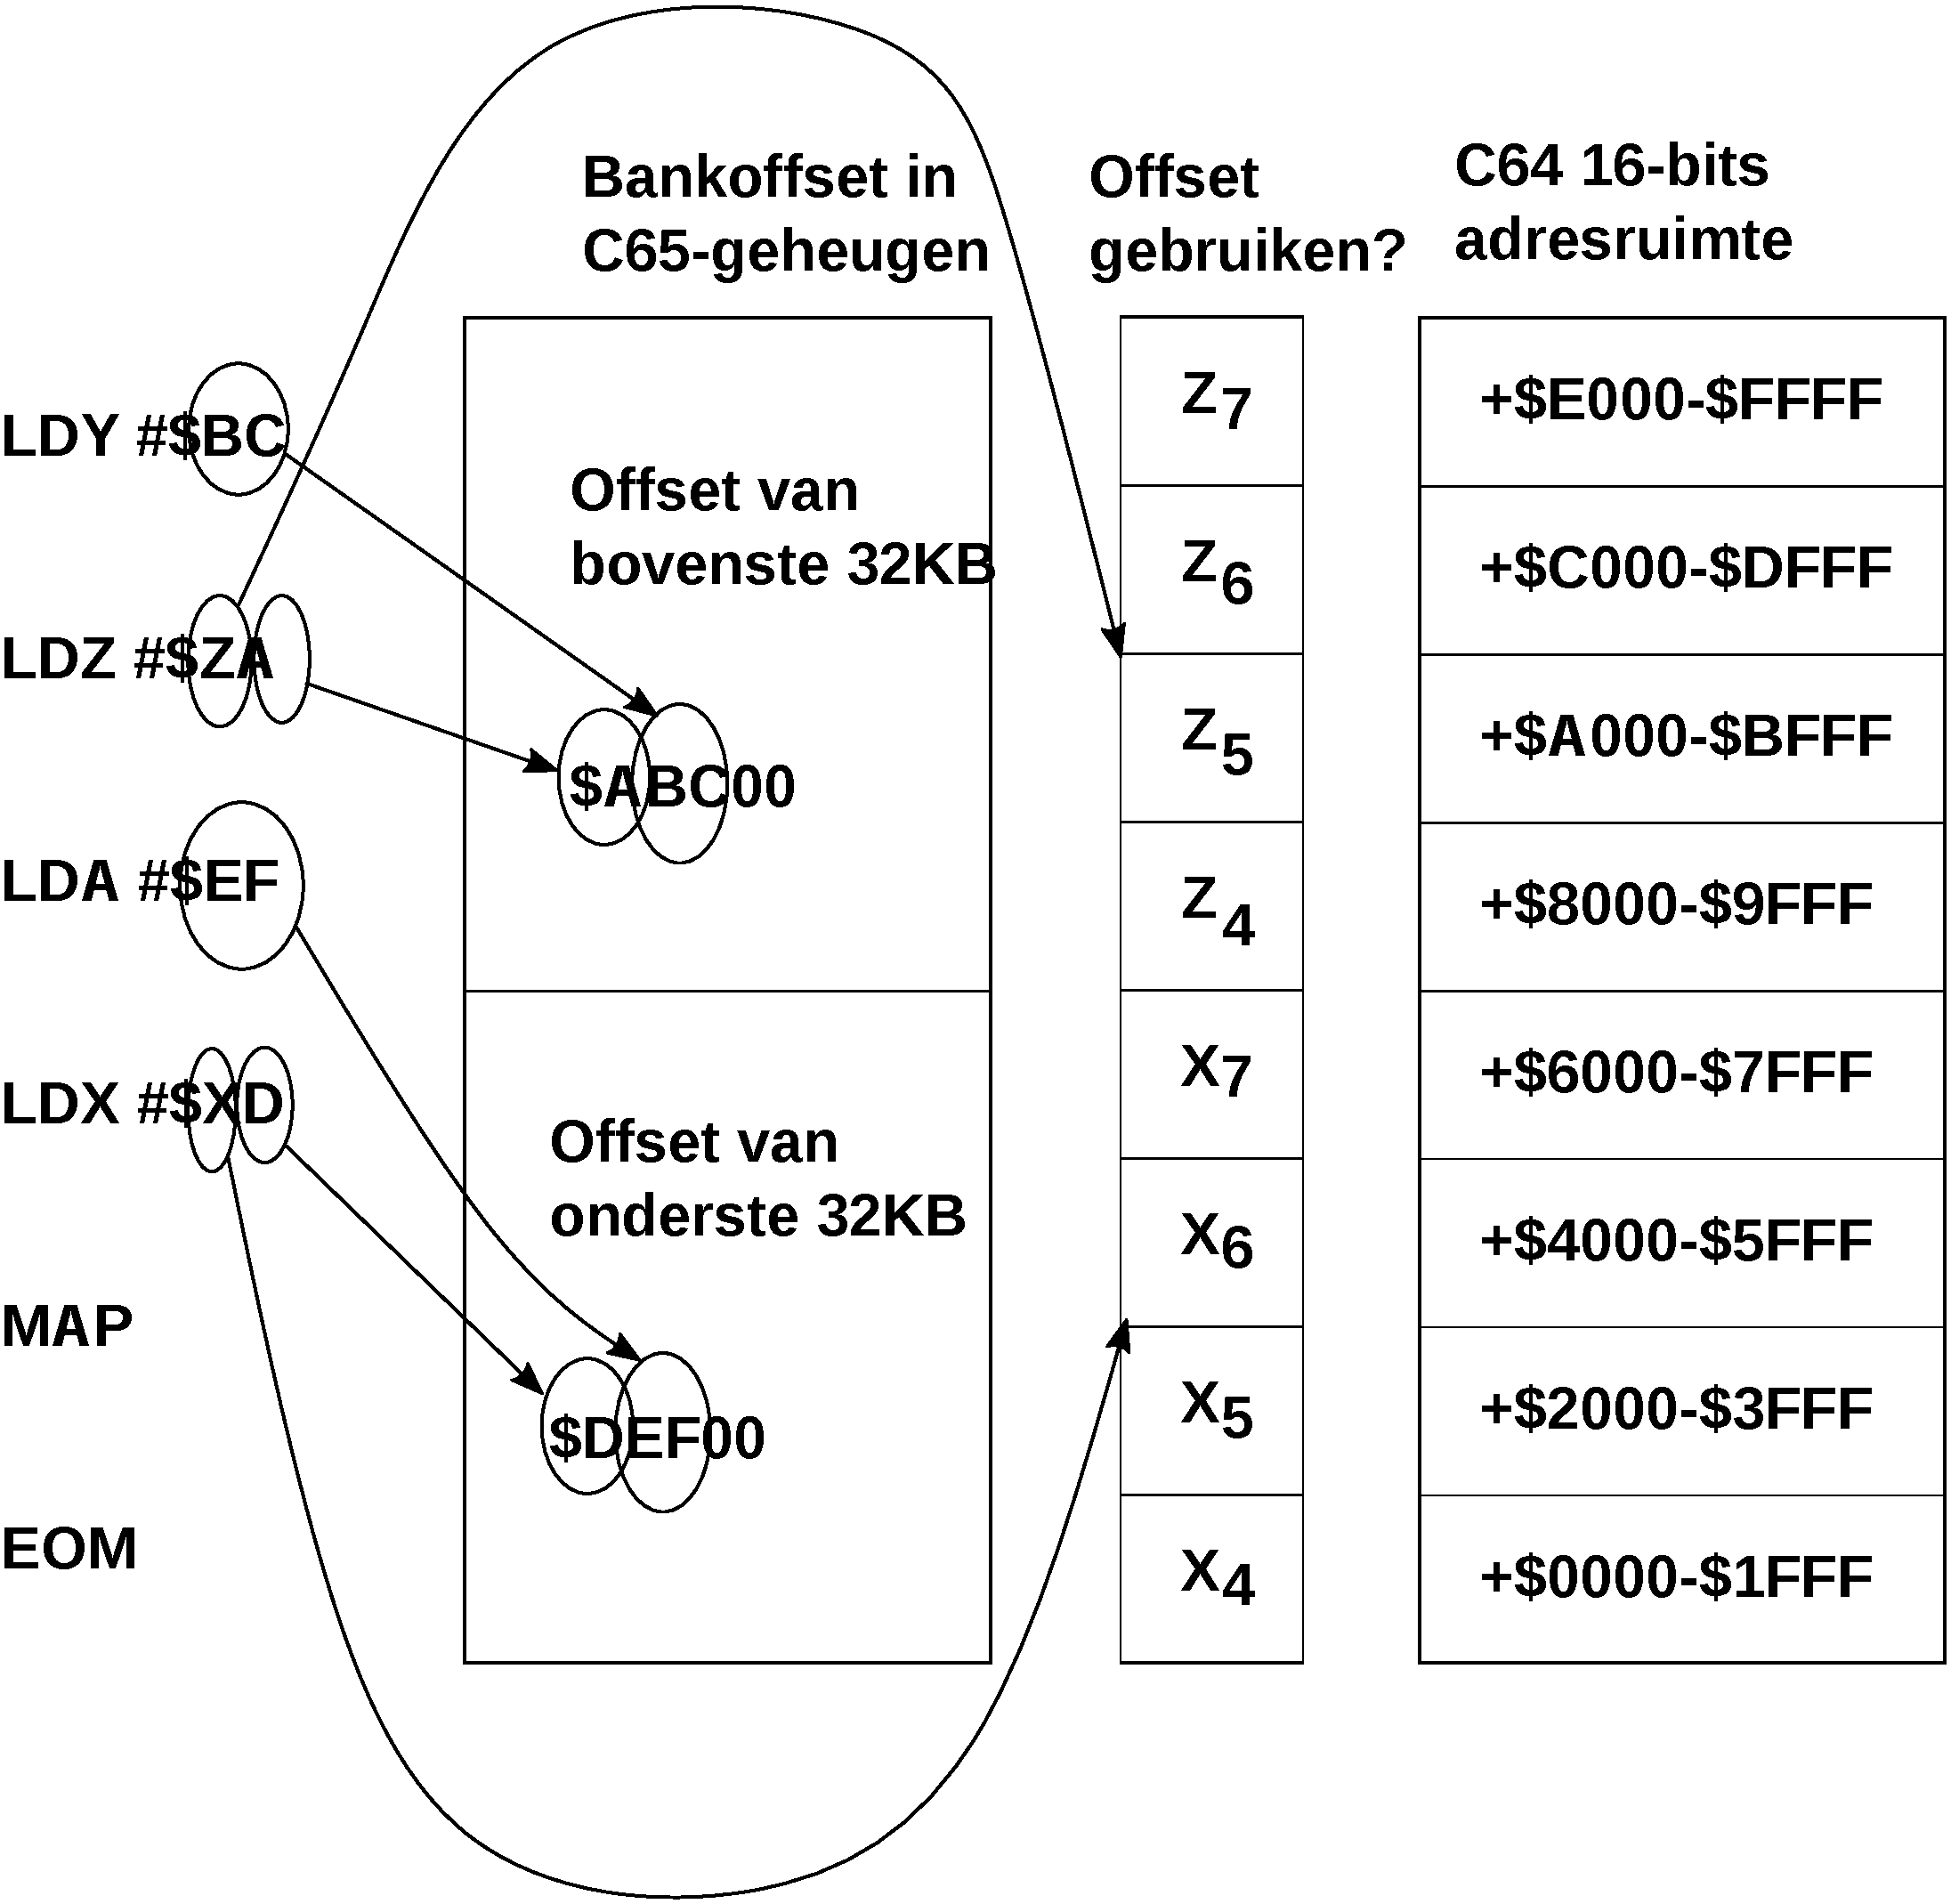
\includegraphics[width=0.75\textwidth]{dutch/images/illustrations/map-instruction-operation.pdf}\index{MAP}\index{Geheugenbanking}
\end{center}

De inhoud van het A-register en de onderste nibble van het X-register vormen samen een 12-bit waarde die met 256 wordt vermenigvuldigd om de offset te produceren die wordt gebruikt voor elk van de 8KB-banken in het onderste 32KB-gedeelte van de 16-bit adresruimte van de 6502. De bovenste nibble van het X-register wordt als vlaggen gebruikt om aan te geven welke van de vier 8KB-blokken in dat 32KB-gedeelte van de 6502-adresruimte de offset bij hun adres moeten optellen om het werkelijke adres te berekenen.

De Y- en Z-registers worden op vergelijkbare manier gebruikt om de offset te produceren voor het bovenste 32KB-gedeelte van de 6502-adresruimte, en de vlaggen om aan te geven of de offset wordt gebruikt voor elk van de vier 8KB-blokken in dat gedeelte van de adresruimte.

De onderste 8 bits van de offset kunnen niet worden ingesteld. De offset is dus een veelvoud van 256 bytes, in tegenstelling tot sommige uitgebreide 6502-processoren. In de praktijk is deze beperking echter zelden van invloed.

Om te begrijpen hoe dit in de praktijk werkt, laat het volgende voorbeeld zien hoe dit werkt met een concreet voorbeeld, met de adresbereiken die zichtbaar zijn in elk van de 8KB-segmenten van de 64KB-adresruimte van de 6502:

\begin{center}
  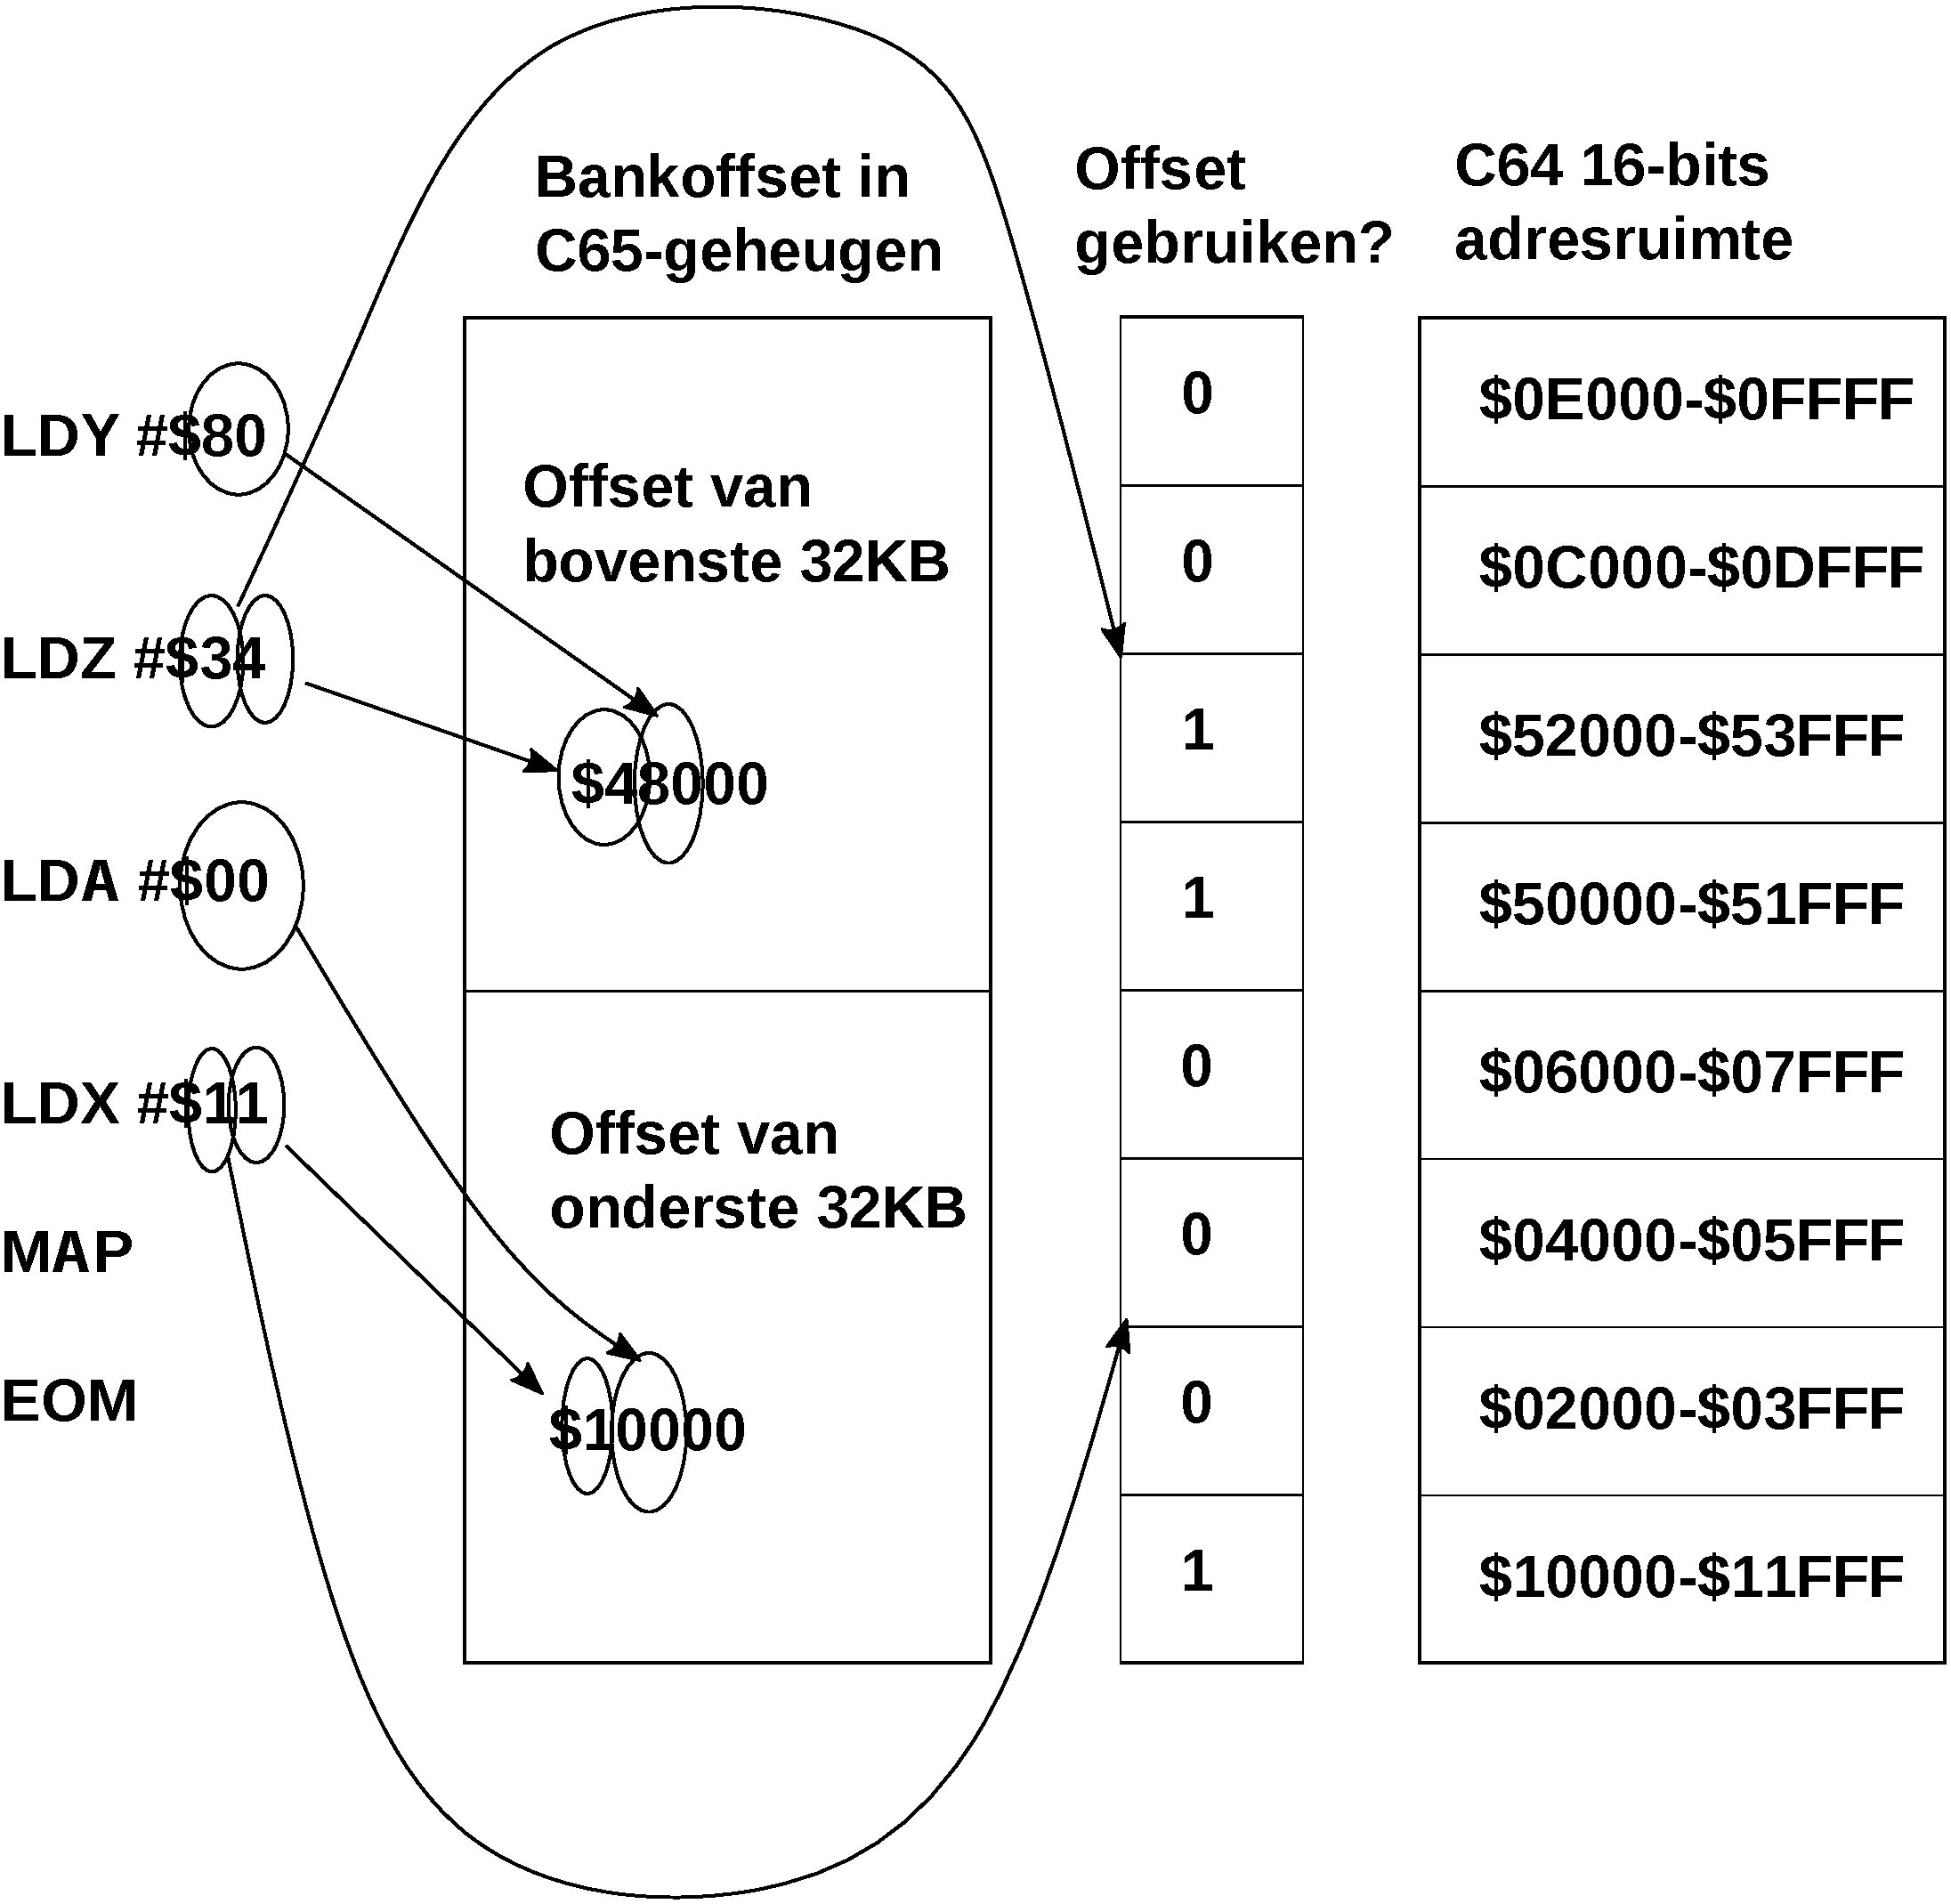
\includegraphics[width=0.75\textwidth]{dutch/images/illustrations/map-instruction-operation-example1.pdf}\index{MAP}\index{Geheugenbanking}
\end{center}

Merk op dat de offsets voor elk van de twee 32KB-adresbereiken worden opgeteld bij het 6502-adres. Vandaar dat de offset van \$48000 voor het bovenste 32KB-gedeelte een adres van \$50000 genereert bij het 6502-adres \$8000.

Zie ook ``De MAP-instructie gebruiken om >1MB te benaderen'' voor verdere uitleg.

\subsubsection{DMA-controller}

De F018/F018A DMA-controller van de C65 maakt het mogelijk om gegevens in het geheugen op willekeurige locaties in de 1MB-adresruimte snel te vullen, te kopiëren en te wisselen. Gedetailleerde informatie over de F018 DMA-controller en de verbeteringen die de MEGA65 daarop heeft aangebracht, vindt u in \bookvref{cha:dmagic}

\subsubsection{Platte geheugentoegang}

\subsection{Toegang tot geheugen buiten het 1MB-punt}
\label{sec:extended-memory}

De MEGA65 kan tot 256MB geheugen ondersteunen. Dit is meer dan de 1MB-adresruimte van de CSG4510 waarop deze is gebaseerd. Er zijn verschillende manieren om dit te bereiken.

\subsubsection{De MAP-instructie gebruiken om >1MB te benaderen}

De volledige adresruimte is beschikbaar voor de MAP-instructie voor traditionele C65-stijl geheugenmapping, hoewel enige voorzichtigheid geboden is, omdat de MAP-instructie tot drie keer moet worden aangeroepen. De reden hiervoor is dat de MAP-instructie eerst moet worden aangeroepen om te selecteren welk megabyte geheugen zal worden gebruikt voor de onderste en bovenste mapregio's, voordat deze opnieuw op de normale manier wordt aangeroepen om de geheugenmapping in te stellen. Omdat tussen deze twee aanroepen de geheugenmapping-offset een mix van oude en nieuwe adressen zal zijn, moet alle mapping eerst worden uitgeschakeld via de MAP-instructie. Dit betekent dat de code voor het hermappen van geheugen zich in het onderste 64KB RAM of in een van de ROM-bankbare regio's moet bevinden, zodat deze tijdens het mappingproces zichtbaar blijft.

Als deze situatie niet goed wordt afgehandeld, zal de processor instructies uitvoeren vanuit een onverwachte geheugenlocatie halverwege het proces, doordat de routine die hij uitvoert om de mapping uit te voeren plotseling niet meer in het geheugen gemapt is.

Vanwege de relatieve complexiteit van dit proces en de andere beperkingen van de MAP-instructie als middel om geheugen te benaderen, raden we u aan om voor gegevens buiten de huidige geheugenindeling ofwel DMA of de flat-memory adresvoorzieningen van de 45GS02 te gebruiken die hieronder worden beschreven. Toegang tot de volledige adresruimte via de MAP-instructie is alleen beschikbaar voor de volledigheid.

Als een ander voorbeeld van hoe de MAP-instructie kan worden gebruikt om een geheugengebied uit de uitgebreide adresruimte te mappen, laat het volgende programma de Ethernet-framebuffer vanaf de natuurlijke locatie op \$FFDE8000 op \$6800 verschijnen. Om het voorbeeld zo eenvoudig mogelijk te houden, gaan we ervan uit dat de code in het onderste 64KB RAM draait en niet in het gebied tussen \$6000 -- \$8000.

Omdat de MAP-instructie normaal gesproken alleen de C65-stijl 20-bit adressen kent, moet de MEGA65-uitbreiding op de instructie worden gebruikt om de bovenste 8 bits van de 28-bit MEGA65-adressen in te stellen, dat wil zeggen welk megabyte adresruimte moet worden gebruikt voor de adresvertaling. Dit wordt gedaan door het X-register in te stellen op \$0F wanneer het megabyte-nummer voor de onderste 32KB van de C64-stijl 64KB-adresruimte wordt gedefinieerd. Dit veroorzaakt geen incompatibiliteit met enig redelijk gebruik van de MAP-instructie op een C65, omdat deze waarde aangeeft dat geen van de vier 8KB-geheugenblokken opnieuw zal worden gemapt, maar tegelijkertijd specificeert dat de bovenste 4 bits van de adresoffset voor het hergemapte blok de niet-nul-waarde \$F vormt. Het megabyte-nummer wordt vervolgens gespecificeerd door het A-register in te stellen.

Dezelfde aanpak geldt voor de bovenste 32KB, maar met de Z- en Y-registers in plaats van de X- en A-registers. In dit geval hoeven we de bovenste 32KB geheugen niet te hermappen; we laten de Z- en Y-registers op nul staan. We moeten echter X en A instellen om het megabyte-nummer voor de onderste 32KB op \$FF te zetten. A moet dus de waarde \$FF hebben. Om de onderste 20 bits van de adresoffset in te stellen, gebruiken we de MAP-instructie een tweede keer, dit keer op de normale C65-manier. Omdat we \$6800 naar \$FFDE800 willen hermappen en al met de \$FFxxxxx-offset via het megabyte-nummer hebben afgerekend, hoeven we alleen de offset toe te passen zodat \$6800 naar \$DE800 wijst. \$DE800 minus \$6800 = \$D8000. Omdat de MAP-instructie werkt met een hermappinggranulariteit van 256 bytes = \$100, kunnen we de laatste twee cijfers van \$D8000 laten vallen om de MAP-offset van \$D80 te verkrijgen. De onderste 8 bits, \$80, moeten in het A-register worden geladen. De bovenste 4 bits, \$D, moeten in de onderste nibble van het X-register worden geladen. Omdat we de mapping alleen op het vierde van de vier 8KB-blokken willen toepassen die de onderste 32KB-helft van de C64-geheugenindeling vormen, moeten we het 4e bit van de bovenste nibble instellen. Dat wil zeggen, de bovenste nibble moet worden ingesteld op \%1000, oftewel \$8. Het X-register moet dus worden geladen met \$8D. Hiermee verkrijgen we het volledige voorbeeldprogramma:

\begin{screencode}
; Map de Ethernet-registers op $6000 - $7FFF

; De Ethernet-controller bevindt zich feitelijk op $FFDE000 - $FFDEFFF, dus selecteer de $FF-megabytesectie voor MAP LO
LDA #$ff
LDX #$0f
LDY #$00
LDZ #$00
map

; Activeer nu het mappen van $DE000-$DFFFF op $6000
; De MAP's zijn op offset gebaseerd, dus moet $6000 van het doeladres worden afgetrokken
; $DE000 - $6000 = $D8000
LDA #$80
LDX #$8d
LDY #$00
LDZ #$00
map
EOM

; De Ethernet-buffer is nu zichtbaar op $6800 - $6FFF
\end{screencode}

De EOM (End Of Mapping)-instructie (hetzelfde als NOP op een 6502, oftewel opcode \$EA) werd alleen na de laatste MAP-instructie opgenomen om er zeker van te zijn dat er geen interrupts konden optreden terwijl de geheugenindeling gemengde waarden bevatte met het megabyte-nummer ingesteld, maar de onderste bits van het mappingadres nog niet waren bijgewerkt.

Er is geen voorbeeld in BASIC voor de MAP-instructie mogelijk, omdat de MAP een machinetaalinstructie is van de 4510/45GS02-processoren.

\subsubsection{Platte geheugentoegang}

De 45GS02 maakt het eenvoudig om een byte vanuit elke geheugenlocatie te lezen of te schrijven door de Zero-Page Indirect-adresseermethode een 32-bit pointer te laten gebruiken in plaats van de gebruikelijke 16-bit pointer. Dit wordt bereikt door de Z-geïndexeerde Zero-Page Indirect-adresseermethode voor de toegang te gebruiken, en de instructie direct te laten voorafgaan door een NOP-instructie (opcode \$EA). Bijvoorbeeld:

\begin{screencode}
NOP
LDA ($45),Z
\end{screencode}

Als u de ACME-assembler of een andere assembler gebruikt die de 45GS02-uitbreidingen ondersteunt, kunt u in plaats daarvan vierkante haakjes gebruiken om aan te geven dat u een flat-memory-bewerking uitvoert. Dergelijke assemblers voegen de \$EA-prefix automatisch voor u in. Bijvoorbeeld:

\begin{screencode}
LDA [$45],Z
\end{screencode}

Ongeacht welk hulpmiddel u gebruikt, in dit voorbeeld zouden de vier bytes Zero-Page-geheugen op \$45 -- \$48 lezen om een 32-bit geheugenadres te vormen, en de waarde van het Z-register hieraan optellen om het werkelijke adres te vormen waaruit wordt gelezen. De bytevolgorde in het adres is hetzelfde als bij de 6502, oftewel het rechtse (minst significante) byte van het adres wordt als eerste gelezen vanaf het eerste adres (\$45 in dit geval), enzovoort, totdat het meest linkse (meest significante) byte wordt gelezen vanaf \$48. Om bijvoorbeeld vanaf geheugenlocatie \$12345678 te lezen, moet de inhoud van het geheugen beginnend op \$45 bestaan uit 78 56 34 12.

Deze methode is veel efficiënter en ook eenvoudiger dan het gebruik van de MAP-instructie of de DMA-controller voor enkelvoudige geheugentoegangen, en is wat wij doorgaans aanbevelen. De DMA-controller kan worden gebruikt voor het verplaatsen/vullen van grotere geheugenregio's. Wij bevelen de MAP-instructie alleen aan voor het banken van code, of in zeldzame situaties waarbij uitgebreide toegang tot een klein geheugengebied vereist is en de extra cycli voor het lezen van de 32-bit-adressen problematisch zijn.

\subsection{Virtueel 32-bit-register}

De 45GS02 maakt het mogelijk om zijn vier algemene registers, A, X, Y en Z (A is LSB, Z is MSB), als één enkel virtueel 32-bit-register te gebruiken, ook wel het {\em Q-pseudoregister} genoemd. Dit kan veelvoorkomende bewerkingen aanzienlijk vereenvoudigen en versnellen, en helpt veelvoorkomende programmeerfouten te voorkomen. Het optellen van twee 16-bit- of 32-bit-waarden kan bijvoorbeeld eenvoudig worden uitgevoerd met iets als:

\begin{screencode}
  ; Wis de carry vóór het optellen, zoals gebruikelijk
  CLC
  ; Laat twee NEG-instructies voorafgaan om de virtuele 32-bit-registermodus te selecteren
  NEG
  NEG
  LDA $1234  ; Laadt de inhoud van $1234-$1237 in respectievelijk A, X, Y en Z
  ; En nogmaals, voor de optelling
  NEG
  NEG
  ADC $1238  ; Telt de inhoud van $1238-$123B op
  ; Het resultaat van de optelling staat nu in A, X, Y en Z.
  ; En kan geheel of gedeeltelijk worden weggeschreven

  ; Om het geheel weg te schrijven is wederom de NEG + NEG-prefix nodig
  NEG
  NEG
  STA $123C ; Schrijft het geheel weg naar $123C-$123F

  ; Of om de laagste bytes weg te schrijven, kan eenvoudigweg de inhoud van A en X normaal worden weggeschreven
  STA $1240
  STX $1241
\end{screencode}

Deze aanpak werkt met de LDA-, STA-, ADC-, SBC-, CMP-, EOR-, AND-, BIT-, ORA-, ASL-, ASR-, LSR-, ROL-, ROR-, INC- en DEC-instructies. Indien u ACME of een andere 45GS02-ondersteunende assembler gebruikt, kunt u in plaats daarvan de nieuwe \stw{LDQ}, \stw{STQ}, \stw{ADCQ}, \stw{SBCQ}, \stw{CPQ}, \stw{EORQ}, \stw{ANDQ}, \stw{BITQ}, \stw{ORQ}, \stw{ASLQ}, \stw{ASRQ}, \stw{LSRQ}, \stw{ROLQ}, \stw{RORQ}, \stw{INQ} en \stw{DEQ} mnemonics gebruiken.\index{LDQ}\index{STQ}\index{ADCQ}\index{SBCQ}\index{CPQ}\index{EORQ}\index{ANDQ}\index{BITQ}\index{ORQ}\index{ASLQ}\index{ASRQ}\index{LSRQ}\index{ROLQ}\index{RORQ}\index{INQ}\index{DEQ} Het vorige voorbeeld wordt dan:

\begin{screencode}
  ; Wis de carry vóór het optellen, zoals gebruikelijk
  CLC
  LDQ  $1234  ; Laadt de inhoud van $1234-$1237 in respectievelijk A, X, Y en Z
  ADCQ $1238  ; Telt de inhoud van $1238-$123B op
  ; Het resultaat van de optelling staat nu in A, X, Y en Z.
  ; En kan geheel of gedeeltelijk worden weggeschreven

  STQ $123C ; Schrijft het geheel weg naar $123C-$123F

  ; Of om de laagste bytes weg te schrijven, kan eenvoudigweg de inhoud van A en X normaal worden weggeschreven
  STA $1240
  STX $1241
\end{screencode}

De virtuele 32-bit-adresseermethode werkt met elke adresseermethode. Geïndexeerde adresseermethoden, waarbij X, Y of Z bij het adres wordt opgeteld, moeten echter met voorzichtigheid worden gebruikt, omdat deze registers in feite een deel van een 32-bit-waarde kunnen bevatten.

De uitzondering is de Zero-Page Indirect Z-geïndexeerde adresseermethode: in dit geval wordt het Z-register NIET bij het doeladres opgeteld (met uitzondering van de LDQ-opcode), in tegenstelling tot wat normaal het geval is. Hierdoor kan het virtuele 32-bit-register worden gebruikt met platte-geheugentoegang met de gecombineerde prefix \stw{NEG NEG NOP} vóór de instructie, zodat een 32-bit-waarde ergens in het geheugen met één instructie kan worden benaderd.

Merk op dat het virtuele 32-bit-register niet kan worden gebruikt in de immediate-modus, bijvoorbeeld om een constante in de vier algemene registers te laden of om een constante waarde op te tellen of af te trekken. Dit dient om problemen met instructies van variabele lengte te voorkomen.

Voor LDQ en STQ bespaart dit hoogstens één byte ten opzichte van LDA \#\$nn ... LDZ \#\$nn, en zou het niet sneller zijn. Voor veel veelvoorkomende waarden, zoals \#\$00000000, bestaan er zelfs verkortingen, zoals:

\begin{screencode}
LDA #$00
TAX
TAY
TAZ
\end{screencode}

Indien u een 32-bit-immediate-waarde moet optellen of aftrekken, kan dit vereisen dat u de argumenten herschikt of andere kleine aanpassingen uitvoert. Om bijvoorbeeld de som van de inhoud van het geheugen en een immediate-waarde te berekenen, kunt u de A-, X-, Y- en Z-registers laden met de immediate-waarde en vervolgens \stw{ADCQ} gebruiken met het geheugenadres:

\begin{screencode}
  ; Haal de immediate-waarde #$12345678 in Q
  LDA #$78
  LDX #$56
  LDY #$34
  LDZ #$12
  ; Telt de inhoud van de geheugenlocaties $1234-$1237 op
  NEG
  NEG
  ADC $1234
  ; Slaat het resultaat op in $1234-$1237
  NEG
  NEG
  STA $1234
\end{screencode}

Wanneer u opnieuw de ACME- of een andere 45GS02-ondersteunende assembler gebruikt, kan dit compacter en duidelijker worden geschreven als volgt. Merk op dat in beide gevallen dezelfde bytevolgorde van machinetaal wordt geproduceerd en het programma hetzelfde aantal cycli zal kosten om uit te voeren.

\begin{screencode}
  ; Haal de immediate-waarde #$12345678 in Q
  LDA #$78
  LDX #$56
  LDY #$34
  LDZ #$12
  ; Telt de inhoud van de geheugenlocaties $1234-$1237 op
  ADCQ $1234
  ; Slaat het resultaat op in $1234-$1237
  STQ $1234
\end{screencode}

\section{In het geheugen gemapte registers van de C64-CPU}

\setlength{\tabcolsep}{0pt}
\begin{longtable}{|C{12.5mm}|C{12.5mm}|C{12.5mm}|C{12.5mm}|C{12.5mm}|C{12.5mm}|C{12.5mm}|C{12.5mm}|C{12.5mm}|C{12.5mm}|}
\hline
{\bf{HEX}} & {\bf{DEC}} & {\bf{DB7}} & {\bf{DB6}} & {\bf{DB5}} & {\bf{DB4}} & {\bf{DB3}} & {\bf{DB2}} & {\bf{DB1}} & {\bf{DB0}} \\
\hline
\endfirsthead
\multicolumn{3}{l@{}}{\ldots Vervolgd}\\
\hline
{\bf{HEX}} & {\bf{DEC}} & {\bf{DB7}} & {\bf{DB6}} & {\bf{DB5}} & {\bf{DB4}} & {\bf{DB3}} & {\bf{DB2}} & {\bf{DB1}} & {\bf{DB0}} \\
\endhead
\multicolumn{3}{l@{}}{Vervolgd \ldots}\\
\endfoot
\hline
\endlastfoot
\footnotesize  00\index{\$00 (PORTDDR)}\index{PORTDDR} & \footnotesize 0 & \multicolumn{8}{c|}{\footnotesize PORTDDR\index{Registers!PORTDDR}}\\
\hline
\footnotesize  01\index{\$01 (C64MAP)}\index{C64MAP} & \footnotesize 1 & \multicolumn{5}{c|}{\footnotesize PORT\index{Registers!PORT}}& \multicolumn{3}{c|}{\footnotesize C64MAP\index{Registers!C64MAP}}\\
\hline
\end{longtable}
\begin{itemize}
\item{\bf{C64MAP}\index{Registers!C64MAP}} Geheugenmapper van de processorport
\item{\bf{PORT}\index{Registers!PORT}} 6510/45GS10 CPU-portgegevens
\item{\bf{PORTDDR}\index{Registers!PORTDDR}} 6510/45GS10 CPU-port-DDR. Schrijf 65 om de 40MHz-modus af te dwingen, of 64 om de normale snelheidscontroles weer in te schakelen.
\end{itemize}


\section{Nieuwe in het geheugen gemapte CPU-registers}

\setlength{\tabcolsep}{0pt}
\begin{longtable}{|C{12.5mm}|C{12.5mm}|C{12.5mm}|C{12.5mm}|C{12.5mm}|C{12.5mm}|C{12.5mm}|C{12.5mm}|C{12.5mm}|C{12.5mm}|}
\hline
{\bf{HEX}} & {\bf{DEC}} & {\bf{DB7}} & {\bf{DB6}} & {\bf{DB5}} & {\bf{DB4}} & {\bf{DB3}} & {\bf{DB2}} & {\bf{DB1}} & {\bf{DB0}} \\
\hline
\endfirsthead
\multicolumn{3}{l@{}}{\ldots Vervolgd}\\
\hline
{\bf{HEX}} & {\bf{DEC}} & {\bf{DB7}} & {\bf{DB6}} & {\bf{DB5}} & {\bf{DB4}} & {\bf{DB3}} & {\bf{DB2}} & {\bf{DB1}} & {\bf{DB0}} \\
\endhead
\multicolumn{3}{l@{}}{Vervolgd \ldots}\\
\endfoot
\hline
\endlastfoot
\footnotesize  D640\index{Registers!\$D640} \index{Registers!54848} & \footnotesize 54848 & \multicolumn{8}{c|}{\footnotesize HTRAP00\index{Registers!HTRAPXX}}\\
\hline
\footnotesize  D641\index{Registers!\$D641} \index{Registers!54849} & \footnotesize 54849 & \multicolumn{8}{c|}{\footnotesize HTRAP01\index{Registers!HTRAP01}}\\
\hline
\footnotesize  D642\index{Registers!\$D642} \index{Registers!54850} & \footnotesize 54850 & \multicolumn{8}{c|}{\footnotesize HTRAP02\index{Registers!HTRAP02}}\\
\hline
\footnotesize  D643\index{Registers!\$D643} \index{Registers!54851} & \footnotesize 54851 & \multicolumn{8}{c|}{\footnotesize HTRAP03\index{Registers!HTRAP03}}\\
\hline
\footnotesize  D644\index{Registers!\$D644} \index{Registers!54852} & \footnotesize 54852 & \multicolumn{8}{c|}{\footnotesize HTRAP04\index{Registers!HTRAP04}}\\
\hline
\footnotesize  D645\index{Registers!\$D645} \index{Registers!54853} & \footnotesize 54853 & \multicolumn{8}{c|}{\footnotesize HTRAP05\index{Registers!HTRAP05}}\\
\hline
\footnotesize  D646\index{Registers!\$D646} \index{Registers!54854} & \footnotesize 54854 & \multicolumn{8}{c|}{\footnotesize HTRAP06\index{Registers!HTRAP06}}\\
\hline
\footnotesize  D647\index{Registers!\$D647} \index{Registers!54855} & \footnotesize 54855 & \multicolumn{8}{c|}{\footnotesize HTRAP07\index{Registers!HTRAP07}}\\
\hline
\footnotesize  D648\index{Registers!\$D648} \index{Registers!54856} & \footnotesize 54856 & \multicolumn{8}{c|}{\footnotesize HTRAP08\index{Registers!HTRAP08}}\\
\hline
\footnotesize  D649\index{Registers!\$D649} \index{Registers!54857} & \footnotesize 54857 & \multicolumn{8}{c|}{\footnotesize HTRAP09\index{Registers!HTRAP09}}\\
\hline
\footnotesize  D64A\index{Registers!\$D64A} \index{Registers!54858} & \footnotesize 54858 & \multicolumn{8}{c|}{\footnotesize HTRAP0A\index{Registers!HTRAP0A}}\\
\hline
\footnotesize  D64B\index{Registers!\$D64B} \index{Registers!54859} & \footnotesize 54859 & \multicolumn{8}{c|}{\footnotesize HTRAP0B\index{Registers!HTRAP0B}}\\
\hline
\footnotesize  D64C\index{Registers!\$D64C} \index{Registers!54860} & \footnotesize 54860 & \multicolumn{8}{c|}{\footnotesize HTRAP0C\index{Registers!HTRAP0C}}\\
\hline
\footnotesize  D64D\index{Registers!\$D64D} \index{Registers!54861} & \footnotesize 54861 & \multicolumn{8}{c|}{\footnotesize HTRAP0D\index{Registers!HTRAP0D}}\\
\hline
\footnotesize  D64E\index{Registers!\$D64E} \index{Registers!54862} & \footnotesize 54862 & \multicolumn{8}{c|}{\footnotesize HTRAP0E\index{Registers!HTRAP0E}}\\
\hline
\footnotesize  D64F\index{Registers!\$D64F} \index{Registers!54863} & \footnotesize 54863 & \multicolumn{8}{c|}{\footnotesize HTRAP0F\index{Registers!HTRAP0F}}\\
\hline
\footnotesize  D650\index{Registers!\$D650} \index{Registers!54864} & \footnotesize 54864 & \multicolumn{8}{c|}{\footnotesize HTRAP10\index{Registers!HTRAP10}}\\
\hline
\footnotesize  D651\index{Registers!\$D651} \index{Registers!54865} & \footnotesize 54865 & \multicolumn{8}{c|}{\footnotesize HTRAP11\index{Registers!HTRAP11}}\\
\hline
\footnotesize  D652\index{Registers!\$D652} \index{Registers!54866} & \footnotesize 54866 & \multicolumn{8}{c|}{\footnotesize HTRAP12\index{Registers!HTRAP12}}\\
\hline
\footnotesize  D653\index{Registers!\$D653} \index{Registers!54867} & \footnotesize 54867 & \multicolumn{8}{c|}{\footnotesize HTRAP13\index{Registers!HTRAP13}}\\
\hline
\footnotesize  D654\index{Registers!\$D654} \index{Registers!54868} & \footnotesize 54868 & \multicolumn{8}{c|}{\footnotesize HTRAP14\index{Registers!HTRAP14}}\\
\hline
\footnotesize  D655\index{Registers!\$D655} \index{Registers!54869} & \footnotesize 54869 & \multicolumn{8}{c|}{\footnotesize HTRAP15\index{Registers!HTRAP15}}\\
\hline
\footnotesize  D656\index{Registers!\$D656} \index{Registers!54870} & \footnotesize 54870 & \multicolumn{8}{c|}{\footnotesize HTRAP16\index{Registers!HTRAP16}}\\
\hline
\footnotesize  D657\index{Registers!\$D657} \index{Registers!54871} & \footnotesize 54871 & \multicolumn{8}{c|}{\footnotesize HTRAP17\index{Registers!HTRAP17}}\\
\hline
\footnotesize  D658\index{Registers!\$D658} \index{Registers!54872} & \footnotesize 54872 & \multicolumn{8}{c|}{\footnotesize HTRAP18\index{Registers!HTRAP18}}\\
\hline
\footnotesize  D659\index{Registers!\$D659} \index{Registers!54873} & \footnotesize 54873 & \multicolumn{8}{c|}{\footnotesize HTRAP19\index{Registers!HTRAP19}}\\
\hline
\footnotesize  D65A\index{Registers!\$D65A} \index{Registers!54874} & \footnotesize 54874 & \multicolumn{8}{c|}{\footnotesize HTRAP1A\index{Registers!HTRAP1A}}\\
\hline
\footnotesize  D65B\index{Registers!\$D65B} \index{Registers!54875} & \footnotesize 54875 & \multicolumn{8}{c|}{\footnotesize HTRAP1B\index{Registers!HTRAP1B}}\\
\hline
\footnotesize  D65C\index{Registers!\$D65C} \index{Registers!54876} & \footnotesize 54876 & \multicolumn{8}{c|}{\footnotesize HTRAP1C\index{Registers!HTRAP1C}}\\
\hline
\footnotesize  D65D\index{Registers!\$D65D} \index{Registers!54877} & \footnotesize 54877 & \multicolumn{8}{c|}{\footnotesize HTRAP1D\index{Registers!HTRAP1D}}\\
\hline
\footnotesize  D65E\index{Registers!\$D65E} \index{Registers!54878} & \footnotesize 54878 & \multicolumn{8}{c|}{\footnotesize HTRAP1E\index{Registers!HTRAP1E}}\\
\hline
\footnotesize  D65F\index{Registers!\$D65F} \index{Registers!54879} & \footnotesize 54879 & \multicolumn{8}{c|}{\footnotesize HTRAP1F\index{Registers!HTRAP1F}}\\
\hline
\footnotesize  D660\index{Registers!\$D660} \index{Registers!54880} & \footnotesize 54880 & \multicolumn{8}{c|}{\footnotesize HTRAP20\index{Registers!HTRAP20}}\\
\hline
\footnotesize  D661\index{Registers!\$D661} \index{Registers!54881} & \footnotesize 54881 & \multicolumn{8}{c|}{\footnotesize HTRAP21\index{Registers!HTRAP21}}\\
\hline
\footnotesize  D662\index{Registers!\$D662} \index{Registers!54882} & \footnotesize 54882 & \multicolumn{8}{c|}{\footnotesize HTRAP22\index{Registers!HTRAP22}}\\
\hline
\footnotesize  D663\index{Registers!\$D663} \index{Registers!54883} & \footnotesize 54883 & \multicolumn{8}{c|}{\footnotesize HTRAP23\index{Registers!HTRAP23}}\\
\hline
\footnotesize  D664\index{Registers!\$D664} \index{Registers!54884} & \footnotesize 54884 & \multicolumn{8}{c|}{\footnotesize HTRAP24\index{Registers!HTRAP24}}\\
\hline
\footnotesize  D665\index{Registers!\$D665} \index{Registers!54885} & \footnotesize 54885 & \multicolumn{8}{c|}{\footnotesize HTRAP25\index{Registers!HTRAP25}}\\
\hline
\footnotesize  D666\index{Registers!\$D666} \index{Registers!54886} & \footnotesize 54886 & \multicolumn{8}{c|}{\footnotesize HTRAP26\index{Registers!HTRAP26}}\\
\hline
\footnotesize  D667\index{Registers!\$D667} \index{Registers!54887} & \footnotesize 54887 & \multicolumn{8}{c|}{\footnotesize HTRAP27\index{Registers!HTRAP27}}\\
\hline
\footnotesize  D668\index{Registers!\$D668} \index{Registers!54888} & \footnotesize 54888 & \multicolumn{8}{c|}{\footnotesize HTRAP28\index{Registers!HTRAP28}}\\
\hline
\footnotesize  D669\index{Registers!\$D669} \index{Registers!54889} & \footnotesize 54889 & \multicolumn{8}{c|}{\footnotesize HTRAP29\index{Registers!HTRAP29}}\\
\hline
\footnotesize  D66A\index{Registers!\$D66A} \index{Registers!54890} & \footnotesize 54890 & \multicolumn{8}{c|}{\footnotesize HTRAP2A\index{Registers!HTRAP2A}}\\
\hline
\footnotesize  D66B\index{Registers!\$D66B} \index{Registers!54891} & \footnotesize 54891 & \multicolumn{8}{c|}{\footnotesize HTRAP2B\index{Registers!HTRAP2B}}\\
\hline
\footnotesize  D66C\index{Registers!\$D66C} \index{Registers!54892} & \footnotesize 54892 & \multicolumn{8}{c|}{\footnotesize HTRAP2C\index{Registers!HTRAP2C}}\\
\hline
\footnotesize  D66D\index{Registers!\$D66D} \index{Registers!54893} & \footnotesize 54893 & \multicolumn{8}{c|}{\footnotesize HTRAP2D\index{Registers!HTRAP2D}}\\
\hline
\footnotesize  D66E\index{Registers!\$D66E} \index{Registers!54894} & \footnotesize 54894 & \multicolumn{8}{c|}{\footnotesize HTRAP2E\index{Registers!HTRAP2E}}\\
\hline
\footnotesize  D66F\index{Registers!\$D66F} \index{Registers!54895} & \footnotesize 54895 & \multicolumn{8}{c|}{\footnotesize HTRAP2F\index{Registers!HTRAP2F}}\\
\hline
\footnotesize  D670\index{Registers!\$D670} \index{Registers!54896} & \footnotesize 54896 & \multicolumn{8}{c|}{\footnotesize HTRAP30\index{Registers!HTRAP30}}\\
\hline
\footnotesize  D671\index{Registers!\$D671} \index{Registers!54897} & \footnotesize 54897 & \multicolumn{8}{c|}{\footnotesize HTRAP31\index{Registers!HTRAP31}}\\
\hline
\footnotesize  D672\index{Registers!\$D672} \index{Registers!54898} & \footnotesize 54898 & \multicolumn{8}{c|}{\footnotesize HTRAP32\index{Registers!HTRAP32}}\\
\hline
\footnotesize  D673\index{Registers!\$D673} \index{Registers!54899} & \footnotesize 54899 & \multicolumn{8}{c|}{\footnotesize HTRAP33\index{Registers!HTRAP33}}\\
\hline
\footnotesize  D674\index{Registers!\$D674} \index{Registers!54900} & \footnotesize 54900 & \multicolumn{8}{c|}{\footnotesize HTRAP34\index{Registers!HTRAP34}}\\
\hline
\footnotesize  D675\index{Registers!\$D675} \index{Registers!54901} & \footnotesize 54901 & \multicolumn{8}{c|}{\footnotesize HTRAP35\index{Registers!HTRAP35}}\\
\hline
\footnotesize  D676\index{Registers!\$D676} \index{Registers!54902} & \footnotesize 54902 & \multicolumn{8}{c|}{\footnotesize HTRAP36\index{Registers!HTRAP36}}\\
\hline
\footnotesize  D677\index{Registers!\$D677} \index{Registers!54903} & \footnotesize 54903 & \multicolumn{8}{c|}{\footnotesize HTRAP37\index{Registers!HTRAP37}}\\
\hline
\footnotesize  D678\index{Registers!\$D678} \index{Registers!54904} & \footnotesize 54904 & \multicolumn{8}{c|}{\footnotesize HTRAP38\index{Registers!HTRAP38}}\\
\hline
\footnotesize  D679\index{Registers!\$D679} \index{Registers!54905} & \footnotesize 54905 & \multicolumn{8}{c|}{\footnotesize HTRAP39\index{Registers!HTRAP39}}\\
\hline
\footnotesize  D67A\index{Registers!\$D67A} \index{Registers!54906} & \footnotesize 54906 & \multicolumn{8}{c|}{\footnotesize HTRAP3A\index{Registers!HTRAP3A}}\\
\hline
\footnotesize  D67B\index{Registers!\$D67B} \index{Registers!54907} & \footnotesize 54907 & \multicolumn{8}{c|}{\footnotesize HTRAP3B\index{Registers!HTRAP3B}}\\
\hline
\footnotesize  D67C\index{Registers!\$D67C} \index{Registers!54908} & \footnotesize 54908 & \multicolumn{8}{c|}{\footnotesize HTRAP3C\index{Registers!HTRAP3C}}\\
\hline
\footnotesize  D67D\index{Registers!\$D67D} \index{Registers!54909} & \footnotesize 54909 & \multicolumn{8}{c|}{\footnotesize HTRAP3D\index{Registers!HTRAP3D}}\\
\hline
\footnotesize  D67E\index{Registers!\$D67E} \index{Registers!54910} & \footnotesize 54910 & \multicolumn{8}{c|}{\footnotesize HTRAP3E\index{Registers!HTRAP3E}}\\
\hline
\footnotesize  D67F\index{Registers!\$D67F} \index{Registers!54911} & \footnotesize 54911 & \multicolumn{8}{c|}{\footnotesize HTRAP3F\index{Registers!HTRAP3F}}\\
\hline
\footnotesize  D710\index{Registers!\$D710} \index{Registers!55056} & \footnotesize 55056 & \multicolumn{2}{c|}{\footnotesize --}& \multicolumn{2}{c|}{\footnotesize BADEXTRA\index{Registers!BADEXTRA}}& \footnotesize BRCOST & \footnotesize -- & \footnotesize SLIEN & \footnotesize BADLEN \\
\hline
\footnotesize  D7EF\index{Registers!\$D7EF} \index{Registers!55279} & \footnotesize 55279 & \multicolumn{8}{c|}{\footnotesize HWRNG\-RAND\index{Registers!HWRNGRAND}}\\
\hline
\footnotesize  D7FA\index{Registers!\$D7FA} \index{Registers!55290} & \footnotesize 55290 & \multicolumn{8}{c|}{\footnotesize FRAMECOUNT\index{Registers!FRAMECOUNT}}\\
\hline
\footnotesize  D7FB\index{Registers!\$D7FB} \index{Registers!55291} & \footnotesize 55291 & \multicolumn{6}{c|}{\footnotesize --}& \footnotesize CARTEN & \footnotesize -- \\
\hline
\footnotesize  D7FD\index{Registers!\$D7FD} \index{Registers!55293} & \footnotesize 55293 & \footnotesize NOEXROM & \footnotesize NOGAME & \multicolumn{5}{c|}{\footnotesize --}& \footnotesize POWEREN \\
\hline
\footnotesize  D7FE\index{Registers!\$D7FE} \index{Registers!55294} & \footnotesize 55294 & \footnotesize HWRNG\-NOTRDY & \footnotesize -- & \footnotesize SLOWSDRAM & \footnotesize SELSDRAM & \footnotesize SLOWCACHE\-ADV & \footnotesize SLOWCACHE & \footnotesize OCEANA & \footnotesize PREFETCH \\
\hline
\end{longtable}
\begin{itemize}
\item{\bf{BADEXTRA}\index{Registers!BADEXTRA}} Kosten van badlines minus 40. D.w.z. 00=40 cycli, 11 = 43 cycli.
\item{\bf{BADLEN}\index{Registers!BADLEN}} Schakelt badline-emulatie in
\item{\bf{BRCOST}\index{Registers!BRCOST}} 1=extra cyclus(sen) rekenen voor genomen vertakkingen
\item{\bf{CARTEN}\index{Registers!CARTEN}} 1=cartridges inschakelen
\item{\bf{FRAMECOUNT}\index{Registers!FRAMECOUNT}} Telt het aantal verstreken videoframes
\item{\bf{HTRAPXX}\index{Registers!HTRAPXX}} Schrijven activeert een hypervisor-trap \$XX
\item{\bf{HWRNGNOTRDY}\index{Registers!HWRNGNOTRDY}} Echte RNG-willekeurig getal van de hardware nog niet gereed (alleen-lezen)
\item{\bf{HWRNGRAND}\index{Registers!HWRNGRAND}} Echt willekeurig getal van de hardware-RNG (lezen activeert de generatie)
\item{\bf{NOEXROM}\index{Registers!NOEXROM}} Overschrijving voor /EXROM: moet 0 zijn om het /EXROM-signaal in te schakelen
\item{\bf{NOGAME}\index{Registers!NOGAME}} Overschrijving voor /GAME: moet 0 zijn om het /GAME-signaal in te schakelen
\item{\bf{OCEANA}\index{Registers!OCEANA}} Schakelt emulatie van cartridge van het type Ocean A in
\item{\bf{POWEREN}\index{Registers!POWEREN}} Zet op nul om de computer uit te schakelen op ondersteunde systemen. ALLEEN-SCHRIJVEN.
\item{\bf{PREFETCH}\index{Registers!PREFETCH}} Schakelt de prefetchlogica voor uitgebreid RAM in
\item{\bf{SELSDRAM}\index{Registers!SELSDRAM}} Selecteert SDRAM in plaats van HyperRAM voor Attic RAM waar beschikbaar
\item{\bf{SLIEN}\index{Registers!SLIEN}} Schakelt interrupts in stijl 6502 (langzaam, 7 cycli) in
\item{\bf{SLOWCACHE}\index{Registers!SLOWCACHE}} Schakelt langzamere regelcaching voor Attic RAM in
\item{\bf{SLOWCACHEADV}\index{Registers!SLOWCACHEADV}} Schakelt de geavanceerde langzamere regelcaching voor Attic RAM in
\item{\bf{SLOWSDRAM}\index{Registers!SLOWSDRAM}} Selecteert de langzame (81MHz) SDRAM-klok
\end{itemize}


\section{MEGA65 CPU-versnellingsregisters voor wiskunde}

Elke MEGA65 bevat een gecombineerde 32-bit-hardwarevermenigvuldiger en -deler. Dit apparaat neemt twee 32-bit-invoeren, {\bf MULTINA} en {\bf MULTINB}, en berekent tegelijkertijd:

\begin{itemize}
\item het 64-bit-product {\bf MULTOUT} van {\bf MULTINA} en {\bf MULTINB}\item het 32-bit-gehele deel {\bf DIVOUT}(4-7) van {\bf MULTINA} gedeeld door {\bf MULTINB}\item het 32-bit-breukdeel {\bf DIVOUT}(0-3) van {\bf MULTINA} gedeeld door {\bf MULTINB}
\end{itemize}

De uitvoer wordt altijd op basis van de invoer bijgewerkt, zodat er geen speciale actie nodig is bij het wijzigen van de invoer. De vermenigvuldiger heeft 1 cyclus nodig om te berekenen, zodat het bijgewerkte resultaat onmiddellijk beschikbaar is (een {\bf MULBUSY}-bit is gedefinieerd, maar deze zal momenteel niet worden gezet). De hardwaredeler kan echter tot 20 cycli kosten, afhankelijk van de specifieke invoer. De programmeur moet de {\bf DIVBUSY}-bit controleren indien de deler nog bezig is met berekenen:

\begin{screencode}
loop:   BIT $D70F   ; brengt de DIVBUSY-bit over naar de N-vlag
        BMI loop    ; zolang deze is gezet, moet worden gewacht
\end{screencode}

De MEGA65 zal ook een programmeerbare rekenunit bevatten, die helpt bij het versnellen van de berekening van vastekommatformules. Deze is momenteel uitgeschakeld en zal verder worden gedocumenteerd zodra deze beschikbaar komt (adressen \$D780 - \$D7E3).

\setlength{\tabcolsep}{0pt}
\begin{longtable}{|C{12.5mm}|C{12.5mm}|C{12.5mm}|C{12.5mm}|C{12.5mm}|C{12.5mm}|C{12.5mm}|C{12.5mm}|C{12.5mm}|C{12.5mm}|}
\hline
{\bf{HEX}} & {\bf{DEC}} & {\bf{DB7}} & {\bf{DB6}} & {\bf{DB5}} & {\bf{DB4}} & {\bf{DB3}} & {\bf{DB2}} & {\bf{DB1}} & {\bf{DB0}} \\
\hline
\endfirsthead
\multicolumn{3}{l@{}}{\ldots Vervolgd}\\
\hline
{\bf{HEX}} & {\bf{DEC}} & {\bf{DB7}} & {\bf{DB6}} & {\bf{DB5}} & {\bf{DB4}} & {\bf{DB3}} & {\bf{DB2}} & {\bf{DB1}} & {\bf{DB0}} \\
\endhead
\multicolumn{3}{l@{}}{Vervolgd \ldots}\\
\endfoot
\hline
\endlastfoot
\footnotesize  D70F\index{Registers!\$D70F} \index{Registers!55055} & \footnotesize 55055 & \footnotesize DIVBUSY & \footnotesize MULBUSY & \multicolumn{6}{c|}{\footnotesize --}\\
\hline
\footnotesize  D768\index{Registers!\$D768} \index{Registers!55144} & \footnotesize 55144 & \multicolumn{8}{c|}{\footnotesize DIVOUT\index{Registers!DIVOUT}}\\
\hline
\footnotesize  D769\index{Registers!\$D769} \index{Registers!55145} & \footnotesize 55145 & \multicolumn{8}{c|}{\footnotesize DIVOUT\index{Registers!DIVOUT}}\\
\hline
\footnotesize  D76A\index{Registers!\$D76A} \index{Registers!55146} & \footnotesize 55146 & \multicolumn{8}{c|}{\footnotesize DIVOUT\index{Registers!DIVOUT}}\\
\hline
\footnotesize  D76B\index{Registers!\$D76B} \index{Registers!55147} & \footnotesize 55147 & \multicolumn{8}{c|}{\footnotesize DIVOUT\index{Registers!DIVOUT}}\\
\hline
\footnotesize  D76C\index{Registers!\$D76C} \index{Registers!55148} & \footnotesize 55148 & \multicolumn{8}{c|}{\footnotesize DIVOUT\index{Registers!DIVOUT}}\\
\hline
\footnotesize  D76D\index{Registers!\$D76D} \index{Registers!55149} & \footnotesize 55149 & \multicolumn{8}{c|}{\footnotesize DIVOUT\index{Registers!DIVOUT}}\\
\hline
\footnotesize  D76E\index{Registers!\$D76E} \index{Registers!55150} & \footnotesize 55150 & \multicolumn{8}{c|}{\footnotesize DIVOUT\index{Registers!DIVOUT}}\\
\hline
\footnotesize  D76F\index{Registers!\$D76F} \index{Registers!55151} & \footnotesize 55151 & \multicolumn{8}{c|}{\footnotesize DIVOUT\index{Registers!DIVOUT}}\\
\hline
\footnotesize  D770\index{Registers!\$D770} \index{Registers!55152} & \footnotesize 55152 & \multicolumn{8}{c|}{\footnotesize MULTINA\index{Registers!MULTINA}}\\
\hline
\footnotesize  D771\index{Registers!\$D771} \index{Registers!55153} & \footnotesize 55153 & \multicolumn{8}{c|}{\footnotesize MULTINA\index{Registers!MULTINA}}\\
\hline
\footnotesize  D772\index{Registers!\$D772} \index{Registers!55154} & \footnotesize 55154 & \multicolumn{8}{c|}{\footnotesize MULTINA\index{Registers!MULTINA}}\\
\hline
\footnotesize  D773\index{Registers!\$D773} \index{Registers!55155} & \footnotesize 55155 & \multicolumn{8}{c|}{\footnotesize MULTINA\index{Registers!MULTINA}}\\
\hline
\footnotesize  D774\index{Registers!\$D774} \index{Registers!55156} & \footnotesize 55156 & \multicolumn{8}{c|}{\footnotesize MULTINB\index{Registers!MULTINB}}\\
\hline
\footnotesize  D775\index{Registers!\$D775} \index{Registers!55157} & \footnotesize 55157 & \multicolumn{8}{c|}{\footnotesize MULTINB\index{Registers!MULTINB}}\\
\hline
\footnotesize  D776\index{Registers!\$D776} \index{Registers!55158} & \footnotesize 55158 & \multicolumn{8}{c|}{\footnotesize MULTINB\index{Registers!MULTINB}}\\
\hline
\footnotesize  D777\index{Registers!\$D777} \index{Registers!55159} & \footnotesize 55159 & \multicolumn{8}{c|}{\footnotesize MULTINB\index{Registers!MULTINB}}\\
\hline
\footnotesize  D778\index{Registers!\$D778} \index{Registers!55160} & \footnotesize 55160 & \multicolumn{8}{c|}{\footnotesize MULTOUT\index{Registers!MULTOUT}}\\
\hline
\footnotesize  D779\index{Registers!\$D779} \index{Registers!55161} & \footnotesize 55161 & \multicolumn{8}{c|}{\footnotesize MULTOUT\index{Registers!MULTOUT}}\\
\hline
\footnotesize  D77A\index{Registers!\$D77A} \index{Registers!55162} & \footnotesize 55162 & \multicolumn{8}{c|}{\footnotesize MULTOUT\index{Registers!MULTOUT}}\\
\hline
\footnotesize  D77B\index{Registers!\$D77B} \index{Registers!55163} & \footnotesize 55163 & \multicolumn{8}{c|}{\footnotesize MULTOUT\index{Registers!MULTOUT}}\\
\hline
\footnotesize  D77C\index{Registers!\$D77C} \index{Registers!55164} & \footnotesize 55164 & \multicolumn{8}{c|}{\footnotesize MULTOUT\index{Registers!MULTOUT}}\\
\hline
\footnotesize  D77D\index{Registers!\$D77D} \index{Registers!55165} & \footnotesize 55165 & \multicolumn{8}{c|}{\footnotesize MULTOUT\index{Registers!MULTOUT}}\\
\hline
\footnotesize  D77E\index{Registers!\$D77E} \index{Registers!55166} & \footnotesize 55166 & \multicolumn{8}{c|}{\footnotesize MULTOUT\index{Registers!MULTOUT}}\\
\hline
\footnotesize  D77F\index{Registers!\$D77F} \index{Registers!55167} & \footnotesize 55167 & \multicolumn{8}{c|}{\footnotesize MULTOUT\index{Registers!MULTOUT}}\\
\hline
\footnotesize  D780\index{Registers!\$D780} \index{Registers!55168} & \footnotesize 55168 & \multicolumn{8}{c|}{\footnotesize MATHIN0\index{Registers!MATHINX}}\\
\hline
\footnotesize  D781\index{Registers!\$D781} \index{Registers!55169} & \footnotesize 55169 & \multicolumn{8}{c|}{\footnotesize MATHIN0\index{Registers!MATHIN0}}\\
\hline
\footnotesize  D782\index{Registers!\$D782} \index{Registers!55170} & \footnotesize 55170 & \multicolumn{8}{c|}{\footnotesize MATHIN0\index{Registers!MATHIN0}}\\
\hline
\footnotesize  D783\index{Registers!\$D783} \index{Registers!55171} & \footnotesize 55171 & \multicolumn{8}{c|}{\footnotesize MATHIN0\index{Registers!MATHIN0}}\\
\hline
\footnotesize  D784\index{Registers!\$D784} \index{Registers!55172} & \footnotesize 55172 & \multicolumn{8}{c|}{\footnotesize MATHIN1\index{Registers!MATHIN1}}\\
\hline
\footnotesize  D785\index{Registers!\$D785} \index{Registers!55173} & \footnotesize 55173 & \multicolumn{8}{c|}{\footnotesize MATHIN1\index{Registers!MATHIN1}}\\
\hline
\footnotesize  D786\index{Registers!\$D786} \index{Registers!55174} & \footnotesize 55174 & \multicolumn{8}{c|}{\footnotesize MATHIN1\index{Registers!MATHIN1}}\\
\hline
\footnotesize  D787\index{Registers!\$D787} \index{Registers!55175} & \footnotesize 55175 & \multicolumn{8}{c|}{\footnotesize MATHIN1\index{Registers!MATHIN1}}\\
\hline
\footnotesize  D788\index{Registers!\$D788} \index{Registers!55176} & \footnotesize 55176 & \multicolumn{8}{c|}{\footnotesize MATHIN2\index{Registers!MATHIN2}}\\
\hline
\footnotesize  D789\index{Registers!\$D789} \index{Registers!55177} & \footnotesize 55177 & \multicolumn{8}{c|}{\footnotesize MATHIN2\index{Registers!MATHIN2}}\\
\hline
\footnotesize  D78A\index{Registers!\$D78A} \index{Registers!55178} & \footnotesize 55178 & \multicolumn{8}{c|}{\footnotesize MATHIN2\index{Registers!MATHIN2}}\\
\hline
\footnotesize  D78B\index{Registers!\$D78B} \index{Registers!55179} & \footnotesize 55179 & \multicolumn{8}{c|}{\footnotesize MATHIN2\index{Registers!MATHIN2}}\\
\hline
\footnotesize  D78C\index{Registers!\$D78C} \index{Registers!55180} & \footnotesize 55180 & \multicolumn{8}{c|}{\footnotesize MATHIN3\index{Registers!MATHIN3}}\\
\hline
\footnotesize  D78D\index{Registers!\$D78D} \index{Registers!55181} & \footnotesize 55181 & \multicolumn{8}{c|}{\footnotesize MATHIN3\index{Registers!MATHIN3}}\\
\hline
\footnotesize  D78E\index{Registers!\$D78E} \index{Registers!55182} & \footnotesize 55182 & \multicolumn{8}{c|}{\footnotesize MATHIN3\index{Registers!MATHIN3}}\\
\hline
\footnotesize  D78F\index{Registers!\$D78F} \index{Registers!55183} & \footnotesize 55183 & \multicolumn{8}{c|}{\footnotesize MATHIN3\index{Registers!MATHIN3}}\\
\hline
\footnotesize  D790\index{Registers!\$D790} \index{Registers!55184} & \footnotesize 55184 & \multicolumn{8}{c|}{\footnotesize MATHIN4\index{Registers!MATHIN4}}\\
\hline
\footnotesize  D791\index{Registers!\$D791} \index{Registers!55185} & \footnotesize 55185 & \multicolumn{8}{c|}{\footnotesize MATHIN4\index{Registers!MATHIN4}}\\
\hline
\footnotesize  D792\index{Registers!\$D792} \index{Registers!55186} & \footnotesize 55186 & \multicolumn{8}{c|}{\footnotesize MATHIN4\index{Registers!MATHIN4}}\\
\hline
\footnotesize  D793\index{Registers!\$D793} \index{Registers!55187} & \footnotesize 55187 & \multicolumn{8}{c|}{\footnotesize MATHIN4\index{Registers!MATHIN4}}\\
\hline
\footnotesize  D794\index{Registers!\$D794} \index{Registers!55188} & \footnotesize 55188 & \multicolumn{8}{c|}{\footnotesize MATHIN5\index{Registers!MATHIN5}}\\
\hline
\footnotesize  D795\index{Registers!\$D795} \index{Registers!55189} & \footnotesize 55189 & \multicolumn{8}{c|}{\footnotesize MATHIN5\index{Registers!MATHIN5}}\\
\hline
\footnotesize  D796\index{Registers!\$D796} \index{Registers!55190} & \footnotesize 55190 & \multicolumn{8}{c|}{\footnotesize MATHIN5\index{Registers!MATHIN5}}\\
\hline
\footnotesize  D797\index{Registers!\$D797} \index{Registers!55191} & \footnotesize 55191 & \multicolumn{8}{c|}{\footnotesize MATHIN5\index{Registers!MATHIN5}}\\
\hline
\footnotesize  D798\index{Registers!\$D798} \index{Registers!55192} & \footnotesize 55192 & \multicolumn{8}{c|}{\footnotesize MATHIN6\index{Registers!MATHIN6}}\\
\hline
\footnotesize  D799\index{Registers!\$D799} \index{Registers!55193} & \footnotesize 55193 & \multicolumn{8}{c|}{\footnotesize MATHIN6\index{Registers!MATHIN6}}\\
\hline
\footnotesize  D79A\index{Registers!\$D79A} \index{Registers!55194} & \footnotesize 55194 & \multicolumn{8}{c|}{\footnotesize MATHIN6\index{Registers!MATHIN6}}\\
\hline
\footnotesize  D79B\index{Registers!\$D79B} \index{Registers!55195} & \footnotesize 55195 & \multicolumn{8}{c|}{\footnotesize MATHIN6\index{Registers!MATHIN6}}\\
\hline
\footnotesize  D79C\index{Registers!\$D79C} \index{Registers!55196} & \footnotesize 55196 & \multicolumn{8}{c|}{\footnotesize MATHIN7\index{Registers!MATHIN7}}\\
\hline
\footnotesize  D79D\index{Registers!\$D79D} \index{Registers!55197} & \footnotesize 55197 & \multicolumn{8}{c|}{\footnotesize MATHIN7\index{Registers!MATHIN7}}\\
\hline
\footnotesize  D79E\index{Registers!\$D79E} \index{Registers!55198} & \footnotesize 55198 & \multicolumn{8}{c|}{\footnotesize MATHIN7\index{Registers!MATHIN7}}\\
\hline
\footnotesize  D79F\index{Registers!\$D79F} \index{Registers!55199} & \footnotesize 55199 & \multicolumn{8}{c|}{\footnotesize MATHIN7\index{Registers!MATHIN7}}\\
\hline
\footnotesize  D7A0\index{Registers!\$D7A0} \index{Registers!55200} & \footnotesize 55200 & \multicolumn{8}{c|}{\footnotesize MATHIN8\index{Registers!MATHIN8}}\\
\hline
\footnotesize  D7A1\index{Registers!\$D7A1} \index{Registers!55201} & \footnotesize 55201 & \multicolumn{8}{c|}{\footnotesize MATHIN8\index{Registers!MATHIN8}}\\
\hline
\footnotesize  D7A2\index{Registers!\$D7A2} \index{Registers!55202} & \footnotesize 55202 & \multicolumn{8}{c|}{\footnotesize MATHIN8\index{Registers!MATHIN8}}\\
\hline
\footnotesize  D7A3\index{Registers!\$D7A3} \index{Registers!55203} & \footnotesize 55203 & \multicolumn{8}{c|}{\footnotesize MATHIN8\index{Registers!MATHIN8}}\\
\hline
\footnotesize  D7A4\index{Registers!\$D7A4} \index{Registers!55204} & \footnotesize 55204 & \multicolumn{8}{c|}{\footnotesize MATHIN9\index{Registers!MATHIN9}}\\
\hline
\footnotesize  D7A5\index{Registers!\$D7A5} \index{Registers!55205} & \footnotesize 55205 & \multicolumn{8}{c|}{\footnotesize MATHIN9\index{Registers!MATHIN9}}\\
\hline
\footnotesize  D7A6\index{Registers!\$D7A6} \index{Registers!55206} & \footnotesize 55206 & \multicolumn{8}{c|}{\footnotesize MATHIN9\index{Registers!MATHIN9}}\\
\hline
\footnotesize  D7A7\index{Registers!\$D7A7} \index{Registers!55207} & \footnotesize 55207 & \multicolumn{8}{c|}{\footnotesize MATHIN9\index{Registers!MATHIN9}}\\
\hline
\footnotesize  D7A8\index{Registers!\$D7A8} \index{Registers!55208} & \footnotesize 55208 & \multicolumn{8}{c|}{\footnotesize MATHINA\index{Registers!MATHINA}}\\
\hline
\footnotesize  D7A9\index{Registers!\$D7A9} \index{Registers!55209} & \footnotesize 55209 & \multicolumn{8}{c|}{\footnotesize MATHINA\index{Registers!MATHINA}}\\
\hline
\footnotesize  D7AA\index{Registers!\$D7AA} \index{Registers!55210} & \footnotesize 55210 & \multicolumn{8}{c|}{\footnotesize MATHINA\index{Registers!MATHINA}}\\
\hline
\footnotesize  D7AB\index{Registers!\$D7AB} \index{Registers!55211} & \footnotesize 55211 & \multicolumn{8}{c|}{\footnotesize MATHINA\index{Registers!MATHINA}}\\
\hline
\footnotesize  D7AC\index{Registers!\$D7AC} \index{Registers!55212} & \footnotesize 55212 & \multicolumn{8}{c|}{\footnotesize MATHINB\index{Registers!MATHINB}}\\
\hline
\footnotesize  D7AD\index{Registers!\$D7AD} \index{Registers!55213} & \footnotesize 55213 & \multicolumn{8}{c|}{\footnotesize MATHINB\index{Registers!MATHINB}}\\
\hline
\footnotesize  D7AE\index{Registers!\$D7AE} \index{Registers!55214} & \footnotesize 55214 & \multicolumn{8}{c|}{\footnotesize MATHINB\index{Registers!MATHINB}}\\
\hline
\footnotesize  D7AF\index{Registers!\$D7AF} \index{Registers!55215} & \footnotesize 55215 & \multicolumn{8}{c|}{\footnotesize MATHINB\index{Registers!MATHINB}}\\
\hline
\footnotesize  D7B0\index{Registers!\$D7B0} \index{Registers!55216} & \footnotesize 55216 & \multicolumn{8}{c|}{\footnotesize MATHINC\index{Registers!MATHINC}}\\
\hline
\footnotesize  D7B1\index{Registers!\$D7B1} \index{Registers!55217} & \footnotesize 55217 & \multicolumn{8}{c|}{\footnotesize MATHINC\index{Registers!MATHINC}}\\
\hline
\footnotesize  D7B2\index{Registers!\$D7B2} \index{Registers!55218} & \footnotesize 55218 & \multicolumn{8}{c|}{\footnotesize MATHINC\index{Registers!MATHINC}}\\
\hline
\footnotesize  D7B3\index{Registers!\$D7B3} \index{Registers!55219} & \footnotesize 55219 & \multicolumn{8}{c|}{\footnotesize MATHINC\index{Registers!MATHINC}}\\
\hline
\footnotesize  D7B4\index{Registers!\$D7B4} \index{Registers!55220} & \footnotesize 55220 & \multicolumn{8}{c|}{\footnotesize MATHIND\index{Registers!MATHIND}}\\
\hline
\footnotesize  D7B5\index{Registers!\$D7B5} \index{Registers!55221} & \footnotesize 55221 & \multicolumn{8}{c|}{\footnotesize MATHIND\index{Registers!MATHIND}}\\
\hline
\footnotesize  D7B6\index{Registers!\$D7B6} \index{Registers!55222} & \footnotesize 55222 & \multicolumn{8}{c|}{\footnotesize MATHIND\index{Registers!MATHIND}}\\
\hline
\footnotesize  D7B7\index{Registers!\$D7B7} \index{Registers!55223} & \footnotesize 55223 & \multicolumn{8}{c|}{\footnotesize MATHIND\index{Registers!MATHIND}}\\
\hline
\footnotesize  D7B8\index{Registers!\$D7B8} \index{Registers!55224} & \footnotesize 55224 & \multicolumn{8}{c|}{\footnotesize MATHINE\index{Registers!MATHINE}}\\
\hline
\footnotesize  D7B9\index{Registers!\$D7B9} \index{Registers!55225} & \footnotesize 55225 & \multicolumn{8}{c|}{\footnotesize MATHINE\index{Registers!MATHINE}}\\
\hline
\footnotesize  D7BA\index{Registers!\$D7BA} \index{Registers!55226} & \footnotesize 55226 & \multicolumn{8}{c|}{\footnotesize MATHINE\index{Registers!MATHINE}}\\
\hline
\footnotesize  D7BB\index{Registers!\$D7BB} \index{Registers!55227} & \footnotesize 55227 & \multicolumn{8}{c|}{\footnotesize MATHINE\index{Registers!MATHINE}}\\
\hline
\footnotesize  D7BC\index{Registers!\$D7BC} \index{Registers!55228} & \footnotesize 55228 & \multicolumn{8}{c|}{\footnotesize MATHINF\index{Registers!MATHINF}}\\
\hline
\footnotesize  D7BD\index{Registers!\$D7BD} \index{Registers!55229} & \footnotesize 55229 & \multicolumn{8}{c|}{\footnotesize MATHINF\index{Registers!MATHINF}}\\
\hline
\footnotesize  D7BE\index{Registers!\$D7BE} \index{Registers!55230} & \footnotesize 55230 & \multicolumn{8}{c|}{\footnotesize MATHINF\index{Registers!MATHINF}}\\
\hline
\footnotesize  D7BF\index{Registers!\$D7BF} \index{Registers!55231} & \footnotesize 55231 & \multicolumn{8}{c|}{\footnotesize MATHINF\index{Registers!MATHINF}}\\
\hline
\footnotesize  D7C0\index{Registers!\$D7C0} \index{Registers!55232} & \footnotesize 55232 & \multicolumn{4}{c|}{\footnotesize UNIT0INB\index{Registers!UNITXINB}}& \multicolumn{4}{c|}{\footnotesize UNIT0INA\index{Registers!UNITXINA}}\\
\hline
\footnotesize  D7C1\index{Registers!\$D7C1} \index{Registers!55233} & \footnotesize 55233 & \multicolumn{4}{c|}{\footnotesize UNIT1INB\index{Registers!UNIT1INB}}& \multicolumn{4}{c|}{\footnotesize UNIT1INA\index{Registers!UNIT1INA}}\\
\hline
\footnotesize  D7C2\index{Registers!\$D7C2} \index{Registers!55234} & \footnotesize 55234 & \multicolumn{4}{c|}{\footnotesize UNIT2INB\index{Registers!UNIT2INB}}& \multicolumn{4}{c|}{\footnotesize UNIT2INA\index{Registers!UNIT2INA}}\\
\hline
\footnotesize  D7C3\index{Registers!\$D7C3} \index{Registers!55235} & \footnotesize 55235 & \multicolumn{4}{c|}{\footnotesize UNIT3INB\index{Registers!UNIT3INB}}& \multicolumn{4}{c|}{\footnotesize UNIT3INA\index{Registers!UNIT3INA}}\\
\hline
\footnotesize  D7C4\index{Registers!\$D7C4} \index{Registers!55236} & \footnotesize 55236 & \multicolumn{4}{c|}{\footnotesize UNIT4INB\index{Registers!UNIT4INB}}& \multicolumn{4}{c|}{\footnotesize UNIT4INA\index{Registers!UNIT4INA}}\\
\hline
\footnotesize  D7C5\index{Registers!\$D7C5} \index{Registers!55237} & \footnotesize 55237 & \multicolumn{4}{c|}{\footnotesize UNIT5INB\index{Registers!UNIT5INB}}& \multicolumn{4}{c|}{\footnotesize UNIT5INA\index{Registers!UNIT5INA}}\\
\hline
\footnotesize  D7C6\index{Registers!\$D7C6} \index{Registers!55238} & \footnotesize 55238 & \multicolumn{4}{c|}{\footnotesize UNIT6INB\index{Registers!UNIT6INB}}& \multicolumn{4}{c|}{\footnotesize UNIT6INA\index{Registers!UNIT6INA}}\\
\hline
\footnotesize  D7C7\index{Registers!\$D7C7} \index{Registers!55239} & \footnotesize 55239 & \multicolumn{4}{c|}{\footnotesize UNIT7INB\index{Registers!UNIT7INB}}& \multicolumn{4}{c|}{\footnotesize UNIT7INA\index{Registers!UNIT7INA}}\\
\hline
\footnotesize  D7C8\index{Registers!\$D7C8} \index{Registers!55240} & \footnotesize 55240 & \multicolumn{4}{c|}{\footnotesize UNIT8INB\index{Registers!UNIT8INB}}& \multicolumn{4}{c|}{\footnotesize UNIT8INA\index{Registers!UNIT8INA}}\\
\hline
\footnotesize  D7C9\index{Registers!\$D7C9} \index{Registers!55241} & \footnotesize 55241 & \multicolumn{4}{c|}{\footnotesize UNIT9INB\index{Registers!UNIT9INB}}& \multicolumn{4}{c|}{\footnotesize UNIT9INA\index{Registers!UNIT9INA}}\\
\hline
\footnotesize  D7CA\index{Registers!\$D7CA} \index{Registers!55242} & \footnotesize 55242 & \multicolumn{4}{c|}{\footnotesize UNITAINB\index{Registers!UNITAINB}}& \multicolumn{4}{c|}{\footnotesize UNITAINA\index{Registers!UNITAINA}}\\
\hline
\footnotesize  D7CB\index{Registers!\$D7CB} \index{Registers!55243} & \footnotesize 55243 & \multicolumn{4}{c|}{\footnotesize UNITBINB\index{Registers!UNITBINB}}& \multicolumn{4}{c|}{\footnotesize UNITBINA\index{Registers!UNITBINA}}\\
\hline
\footnotesize  D7CC\index{Registers!\$D7CC} \index{Registers!55244} & \footnotesize 55244 & \multicolumn{4}{c|}{\footnotesize UNITCINB\index{Registers!UNITCINB}}& \multicolumn{4}{c|}{\footnotesize UNITCINA\index{Registers!UNITCINA}}\\
\hline
\footnotesize  D7CD\index{Registers!\$D7CD} \index{Registers!55245} & \footnotesize 55245 & \multicolumn{4}{c|}{\footnotesize UNITDINB\index{Registers!UNITDINB}}& \multicolumn{4}{c|}{\footnotesize UNITDINA\index{Registers!UNITDINA}}\\
\hline
\footnotesize  D7CE\index{Registers!\$D7CE} \index{Registers!55246} & \footnotesize 55246 & \multicolumn{4}{c|}{\footnotesize UNITEINB\index{Registers!UNITEINB}}& \multicolumn{4}{c|}{\footnotesize UNITEINA\index{Registers!UNITEINA}}\\
\hline
\footnotesize  D7CF\index{Registers!\$D7CF} \index{Registers!55247} & \footnotesize 55247 & \multicolumn{4}{c|}{\footnotesize UNITFINB\index{Registers!UNITFINB}}& \multicolumn{4}{c|}{\footnotesize UNITFINA\index{Registers!UNITFINA}}\\
\hline
\footnotesize  D7D0\index{Registers!\$D7D0} \index{Registers!55248} & \footnotesize 55248 & \footnotesize U0\-LATCH & \footnotesize U0\-MLADD & \footnotesize U0\-HIOUT & \footnotesize U0\-LOWOUT & \multicolumn{4}{c|}{\footnotesize UNIT0OUT\index{Registers!UNITXOUT}}\\
\hline
\footnotesize  D7D1\index{Registers!\$D7D1} \index{Registers!55249} & \footnotesize 55249 & \footnotesize U1\-LATCH & \footnotesize U1\-MLADD & \footnotesize U1\-HIOUT & \footnotesize U1\-LOWOUT & \multicolumn{4}{c|}{\footnotesize UNIT1OUT\index{Registers!UNIT1OUT}}\\
\hline
\footnotesize  D7D2\index{Registers!\$D7D2} \index{Registers!55250} & \footnotesize 55250 & \footnotesize U2\-LATCH & \footnotesize U2\-MLADD & \footnotesize U2\-HIOUT & \footnotesize U2\-LOWOUT & \multicolumn{4}{c|}{\footnotesize UNIT2OUT\index{Registers!UNIT2OUT}}\\
\hline
\footnotesize  D7D3\index{Registers!\$D7D3} \index{Registers!55251} & \footnotesize 55251 & \footnotesize U3\-LATCH & \footnotesize U3\-MLADD & \footnotesize U3\-HIOUT & \footnotesize U3\-LOWOUT & \multicolumn{4}{c|}{\footnotesize UNIT3OUT\index{Registers!UNIT3OUT}}\\
\hline
\footnotesize  D7D4\index{Registers!\$D7D4} \index{Registers!55252} & \footnotesize 55252 & \footnotesize U4\-LATCH & \footnotesize U4\-MLADD & \footnotesize U4\-HIOUT & \footnotesize U4\-LOWOUT & \multicolumn{4}{c|}{\footnotesize UNIT4OUT\index{Registers!UNIT4OUT}}\\
\hline
\footnotesize  D7D5\index{Registers!\$D7D5} \index{Registers!55253} & \footnotesize 55253 & \footnotesize U5\-LATCH & \footnotesize U5\-MLADD & \footnotesize U5\-HIOUT & \footnotesize U5\-LOWOUT & \multicolumn{4}{c|}{\footnotesize UNIT5OUT\index{Registers!UNIT5OUT}}\\
\hline
\footnotesize  D7D6\index{Registers!\$D7D6} \index{Registers!55254} & \footnotesize 55254 & \footnotesize U6\-LATCH & \footnotesize U6\-MLADD & \footnotesize U6\-HIOUT & \footnotesize U6\-LOWOUT & \multicolumn{4}{c|}{\footnotesize UNIT6OUT\index{Registers!UNIT6OUT}}\\
\hline
\footnotesize  D7D7\index{Registers!\$D7D7} \index{Registers!55255} & \footnotesize 55255 & \footnotesize U7\-LATCH & \footnotesize U7\-MLADD & \footnotesize U7\-HIOUT & \footnotesize U7\-LOWOUT & \multicolumn{4}{c|}{\footnotesize UNIT7OUT\index{Registers!UNIT7OUT}}\\
\hline
\footnotesize  D7D8\index{Registers!\$D7D8} \index{Registers!55256} & \footnotesize 55256 & \footnotesize U8\-LATCH & \footnotesize U8\-BSADD & \footnotesize U8\-HIOUT & \footnotesize U8\-LOWOUT & \multicolumn{4}{c|}{\footnotesize UNIT8OUT\index{Registers!UNIT8OUT}}\\
\hline
\footnotesize  D7D9\index{Registers!\$D7D9} \index{Registers!55257} & \footnotesize 55257 & \footnotesize U9\-LATCH & \footnotesize U9\-BSADD & \footnotesize U9\-HIOUT & \footnotesize U9\-LOWOUT & \multicolumn{4}{c|}{\footnotesize UNIT9OUT\index{Registers!UNIT9OUT}}\\
\hline
\footnotesize  D7DA\index{Registers!\$D7DA} \index{Registers!55258} & \footnotesize 55258 & \footnotesize UA\-LATCH & \footnotesize UA\-BSADD & \footnotesize UA\-HIOUT & \footnotesize UA\-LOWOUT & \multicolumn{4}{c|}{\footnotesize UNITAOUT\index{Registers!UNITAOUT}}\\
\hline
\footnotesize  D7DB\index{Registers!\$D7DB} \index{Registers!55259} & \footnotesize 55259 & \footnotesize UB\-LATCH & \footnotesize UB\-BSADD & \footnotesize UB\-HIOUT & \footnotesize UB\-LOWOUT & \multicolumn{4}{c|}{\footnotesize UNITBOUT\index{Registers!UNITBOUT}}\\
\hline
\footnotesize  D7DC\index{Registers!\$D7DC} \index{Registers!55260} & \footnotesize 55260 & \footnotesize UC\-LATCH & \footnotesize UC\-DVADD & \footnotesize UC\-HIOUT & \footnotesize UC\-LOWOUT & \multicolumn{4}{c|}{\footnotesize UNITCOUT\index{Registers!UNITCOUT}}\\
\hline
\footnotesize  D7DD\index{Registers!\$D7DD} \index{Registers!55261} & \footnotesize 55261 & \footnotesize UD\-LATCH & \footnotesize UD\-DVADD & \footnotesize UD\-HIOUT & \footnotesize UD\-LOWOUT & \multicolumn{4}{c|}{\footnotesize UNITDOUT\index{Registers!UNITDOUT}}\\
\hline
\footnotesize  D7DE\index{Registers!\$D7DE} \index{Registers!55262} & \footnotesize 55262 & \footnotesize UE\-LATCH & \footnotesize UE\-DVADD & \footnotesize UE\-HIOUT & \footnotesize UE\-LOWOUT & \multicolumn{4}{c|}{\footnotesize UNITEOUT\index{Registers!UNITEOUT}}\\
\hline
\footnotesize  D7DF\index{Registers!\$D7DF} \index{Registers!55263} & \footnotesize 55263 & \footnotesize UF\-LATCH & \footnotesize UF\-DVADD & \footnotesize UF\-HIOUT & \footnotesize UF\-LOWOUT & \multicolumn{4}{c|}{\footnotesize UNITFOUT\index{Registers!UNITFOUT}}\\
\hline
\footnotesize  D7E0\index{Registers!\$D7E0} \index{Registers!55264} & \footnotesize 55264 & \multicolumn{8}{c|}{\footnotesize LATCHINT\index{Registers!LATCHINT}}\\
\hline
\footnotesize  D7E1\index{Registers!\$D7E1} \index{Registers!55265} & \footnotesize 55265 & \multicolumn{6}{c|}{\footnotesize --}& \footnotesize CALCEN & \footnotesize WREN \\
\hline
\footnotesize  D7E2\index{Registers!\$D7E2} \index{Registers!55266} & \footnotesize 55266 & \multicolumn{8}{c|}{\footnotesize RESERVED\index{Registers!RESERVED}}\\
\hline
\footnotesize  D7E3\index{Registers!\$D7E3} \index{Registers!55267} & \footnotesize 55267 & \multicolumn{8}{c|}{\footnotesize RESERVED\index{Registers!RESERVED}}\\
\hline
\end{longtable}
\begin{itemize}
\item{\bf{CALCEN}\index{Registers!CALCEN}} Maakt het vastleggen van uitvoerwaarden van rekenunits in de wiskunderegisters mogelijk (uitwissen pauzeert effectief iteratieve formules)
\item{\bf{DIVBUSY}\index{Registers!DIVBUSY}} Gezet indien de hardwaredeler bezig is
\item{\bf{DIVOUT}\index{Registers!DIVOUT}} 64-bit-uitvoer van MULTINA $\div$ MULTINB
\item{\bf{LATCHINT}\index{Registers!LATCHINT}} Vastleginterval voor vastgelegde uitvoer (in CPU-cycli)
\item{\bf{MATHINX}\index{Registers!MATHINX}} 32-bit-invoer X van de rekenunit
\item{\bf{MULBUSY}\index{Registers!MULBUSY}} Gezet indien de hardwarevermenigvuldiger bezig is
\item{\bf{MULTINA}\index{Registers!MULTINA}} Vermenigvuldiger-invoer A / teller van de deler (32 bit)
\item{\bf{MULTINB}\index{Registers!MULTINB}} Vermenigvuldiger-invoer B / noemer van de deler (32 bit)
\item{\bf{MULTOUT}\index{Registers!MULTOUT}} 64-bit-uitvoer van MULTINA $\times$ MULTINB
\item{\bf{RESERVED}\index{Registers!RESERVED}} Gereserveerd
\item{\bf{UNITXINA}\index{Registers!UNITXINA}} Selecteert welke van de 16 32-bit-wiskunderegisters invoer A is voor rekenfunctieunit X.
\item{\bf{UNITXINB}\index{Registers!UNITXINB}} Selecteert welke van de 16 32-bit-wiskunderegisters invoer B is voor rekenfunctieunit X.
\item{\bf{UNITXOUT}\index{Registers!UNITXOUT}} Selecteert welke van de 16 32-bit-wiskunderegisters de uitvoer van rekenfunctieunit X ontvangt
\item{\bf{UXBSADD}\index{Registers!UXBSADD}} Indien gezet, treedt rekenfunctieunit Y op als een 32-bit-opteller in plaats van een 32-bit-barrelshifter.
\item{\bf{UXDVADD}\index{Registers!UXDVADD}} Indien gezet, treedt rekenfunctieunit X op als een 32-bit-opteller in plaats van een 32-bit-deler.
\item{\bf{UXHIOUT}\index{Registers!UXHIOUT}} Indien gezet, wordt de hoge helft van de uitvoer van rekenfunctieunit X naar het wiskunderegister UNITXOUT geschreven.
\item{\bf{UXLATCH}\index{Registers!UXLATCH}} Indien gezet, wordt de uitvoer van rekenfunctieunit X vastgelegd.
\item{\bf{UXLOWOUT}\index{Registers!UXLOWOUT}} Indien gezet, wordt de lage helft van de uitvoer van rekenfunctieunit X naar het wiskunderegister UNITXOUT geschreven.
\item{\bf{UXMLADD}\index{Registers!UXMLADD}} Indien gezet, treedt rekenfunctieunit X op als een 32-bit-opteller in plaats van een 32-bit-vermenigvuldiger.
\item{\bf{WREN}\index{Registers!WREN}} Maakt het instellen van de wiskunderegisters mogelijk (moet normaal gezet zijn)
\end{itemize}


\section{MEGA65-hypervisormodus}
\label{sec:hypervisor-mode}

\subsection{Reset}

Bij inschakeling of reset start de MEGA65 in de hypervisormodus op en verwacht een programma in het 16KB-hypervisorgeheugen, en begint het uitvoeren van instructies op adres \$8100. Normaal bevindt zich op dit adres een JMP-instructie die naar een routine voor reset springt. Dat wil zeggen, de 45GS02 gebruikt niet de normale resetvector van de 6502. De functie daarvan wordt geëmuleerd door het Hyppo-hypervisorprogramma, dat het adres ophaalt uit de resetvector van de 6502 in het geladen clientbesturingssysteem wanneer het de hypervisormodus verlaat.

Het hypervisorgeheugen wordt bij reset automatisch op \$8000 - \$BFFF gemapt. Dit speciale geheugen kan niet worden gemapt of op enige andere manier worden benaderd, behalve wanneer de processor zich in de hypervisormodus bevindt. Het kan echter altijd worden benaderd vanuit de seriële monitor-/debuggerinterface via zijn 28-bit-adres, \$FFF8000 -- \$FFFBFFF. Dit beschermt het tegen onbedoelde of kwaadwillende toegang vanuit een gastbesturingssysteem.

\subsection{De hypervisormodus in- en uitstappen}

Het betreden van de hypervisor vindt plaats wanneer een van de volgende gebeurtenissen optreedt:

\begin{itemize}
\item{\bf Inschakelen} Wanneer de MEGA65 voor het eerst wordt ingeschakeld.\item{\bf Reset} Wanneer de resetlijn laag wordt gemaakt of een reset door een watchdog wordt geactiveerd.\item{\bf SYSCALL-register benaderd} De registers \$D640 - \$D67F in de MEGA65 I/O-modus activeren SYSCALLs wanneer ze worden benaderd. Dit is bedoeld als het mechanisme waarmee een clientbesturingssysteem of -proces de aandacht van de hypervisor of het besturingssysteem verzoekt.\item{\bf Paginafout} Op MEGA65's met virtueel geheugen veroorzaakt een paginafout een trap naar de hypervisormodus.\item{\bf Bepaalde toetsenbordgebeurtenissen} Het langer dan 0.5 seconden ingedrukt houden van \widekey{RESTORE}, of de combinatie van de \megasymbolkey- en \specialkey{TAB}-toets, activeert een trap naar de hypervisor. Doorgaans wordt het eerste gebruikt om het Freeze-menu te starten en het tweede om de weergave van de debuginterface te wisselen.\item{\bf Benaderen van virtueel gemaakte I/O-apparaten} Indien bijvoorbeeld de F011 (interne 3.5''-schijfstationcontroller) is gevirtualiseerd, zal het pogingen om sectoren met dit apparaat te lezen of schrijven activeren tot trappen naar de hypervisor. \item{\bf Uitvoeren van een instructie die de CPU zou blokkeren} Een aantal niet-gedocumenteerde opcodes op de 6502 zal de CPU blokkeren. Op de MEGA65 zal de computer in plaats daarvan een trap naar de hypervisor activeren. Dit kan worden gebruikt om alternatieve instructiegedragingen te implementeren, of eenvoudigweg om de gebruiker te melden dat er iets fout is gegaan. \item{\bf Bepaalde speciale gebeurtenissen} Sommige apparaten kunnen hypervisor-niveau-onderbrekingen genereren. Deze worden geïmplementeerd als trappen naar de hypervisor.
\end{itemize}

De 45GS02 verwerkt al deze gebeurtenissen op een vergelijkbare manier intern:

\begin{enumerate}
\item Het SYSCALL- of trap-adres wordt berekend, op basis van de gebeurtenis.\item De inhoud van alle CPU-registers wordt opgeslagen in de virtualisatiebesturingsregisters.\item De geheugenindeling van de hypervisormodus wordt geactiveerd, de decimale vlag van de CPU en de special purpose-registers worden allemaal op geschikte waarden gezet.  De inhoud van de A-, X-, Y- en Z-registers en de meeste andere CPU-vlaggen blijven behouden, zodat die benaderd kunnen worden vanuit de SYSCALL/trap-handlerroutine van de hypervisor, zonder ze te moeten laden, wat een paar cycli per aanroep bespaart.\item De hypervisormodus-vlag wordt gezet en de programmateller (PC) wordt op het berekende adres gezet.
\end{enumerate}

Al het bovenstaande gebeurt in één CPU-cyclus, d.w.z. in 25 nanoseconden. Terugkeren van een SYSCALL of trap bestaat eenvoudigweg uit het schrijven naar \$D67F, wat 125 nanoseconden vereist, voor een totale overhead van 150 nanoseconden. Dit geeft de SYSCALL-prestaties van de MEGA65 die wedijveren met -- zelfs sneller zijn dan -- zelfs de snelste moderne computers, waar de systeemaanroeplatentie doorgaans honderden tot tienduizenden cycli bedraagt \cite{soares2010flexsc}.

\subsection{Hypervisor-geheugenindeling}

Het hypervisorgeheugen heeft een grootte van 16KB. De eerste 512 bytes zijn gereserveerd voor SYSCALL- en systeem-trap-ingangspunten, met vier bytes voor elk. Het reset-ingangspunt is bijvoorbeeld \$8100 - \$8100 + 3 = \$8100 - \$8103. Dit laat 4 bytes toe voor een instructie, doorgaans een JMP-instructie, gevolgd door een NOP om deze tot 4 bytes op te vullen.

De volledige lijst van SYSCALLs en traps is:

\begin{longtable}{|L{1.2cm}|L{1.1cm}|C{2cm}|L{6cm}|}
\hline
{\bf{HEX}} & {\bf{DEC}} & {\bf{Naam}} & {\bf{Omschrijving}} \\
\hline
\endfirsthead
\multicolumn{3}{l@{}}{\ldots Vervolgd}\\
\hline
{\bf{HEX}} & {\bf{DEC}} & {\bf{Naam}} & {\bf{Omschrijving}} \\
\hline
\endhead
\multicolumn{3}{l@{}}{Vervolgd \ldots}\\
\endfoot
\hline
\endlastfoot
\small  8000 & \small 32768 & SYSCALL00 & SYSCALL 0 ingangspunt \\
\hline
\small  8004 & \small 32772 & SYSCALL01 & SYSCALL 1 ingangspunt \\
\hline
\small  8008 & \small 32776 & SYSCALL02 & SYSCALL 2 ingangspunt \\
\hline
\small  800C & \small 32780 & SYSCALL03 & SYSCALL 3 ingangspunt \\
\hline
\small  8010 & \small 32784 & SYSCALL04 & SYSCALL 4 ingangspunt \\
\hline
\small  8014 & \small 32788 & SYSCALL05 & SYSCALL 5 ingangspunt \\
\hline
\small  8018 & \small 32792 & SYSCALL06 & SYSCALL 6 ingangspunt \\
\hline
\small  801C & \small 32796 & SYSCALL07 & SYSCALL 7 ingangspunt \\
\hline
\small  8020 & \small 32800 & SYSCALL08 & SYSCALL 8 ingangspunt \\
\hline
\small  8024 & \small 32804 & SYSCALL09 & SYSCALL 9 ingangspunt \\
\hline
\small  8028 & \small 32808 & SYSCALL0A & SYSCALL 10 ingangspunt \\
\hline
\small  802C & \small 32812 & SYSCALL0B & SYSCALL 11 ingangspunt \\
\hline
\small  8030 & \small 32816 & SYSCALL0C & SYSCALL 12 ingangspunt \\
\hline
\small  8034 & \small 32820 & SYSCALL0D & SYSCALL 13 ingangspunt \\
\hline
\small  8038 & \small 32824 & SYSCALL0E & SYSCALL 14 ingangspunt \\
\hline
\small  803C & \small 32828 & SYSCALL0F & SYSCALL 15 ingangspunt \\
\hline
\small  8040 & \small 32832 & SYSCALL10 & SYSCALL 16 ingangspunt \\
\hline
\small  8044 & \small 32836 & SECURENTR & Ingangspunt van de trap naar de beveiligde container \\
\hline
\small  8048 & \small 32840 & SECUREXIT & Verlaten van de beveiligde container trap-ingangspunt. \\
\hline
\small  804C & \small 32844 & SYSCALL13 & SYSCALL 19 ingangspunt \\
\hline
\small  8050 & \small 32848 & SYSCALL14 & SYSCALL 20 ingangspunt \\
\hline
\small  8054 & \small 32852 & SYSCALL15 & SYSCALL 21 ingangspunt \\
\hline
\small  8058 & \small 32856 & SYSCALL16 & SYSCALL 22 ingangspunt \\
\hline
\small  805C & \small 32860 & SYSCALL17 & SYSCALL 23 ingangspunt \\
\hline
\small  8060 & \small 32864 & SYSCALL18 & SYSCALL 24 ingangspunt \\
\hline
\small  8064 & \small 32868 & SYSCALL19 & SYSCALL 25 ingangspunt \\
\hline
\small  8068 & \small 32872 & SYSCALL1A & SYSCALL 26 ingangspunt \\
\hline
\small  806C & \small 32876 & SYSCALL1B & SYSCALL 27 ingangspunt \\
\hline
\small  8070 & \small 32880 & SYSCALL1C & SYSCALL 28 ingangspunt \\
\hline
\small  8074 & \small 32884 & SYSCALL1D & SYSCALL 29 ingangspunt \\
\hline
\small  8078 & \small 32888 & SYSCALL1E & SYSCALL 30 ingangspunt \\
\hline
\small  807C & \small 32892 & SYSCALL1F & SYSCALL 31 ingangspunt \\
\hline
\small  8080 & \small 32896 & SYSCALL20 & SYSCALL 32 ingangspunt \\
\hline
\small  8084 & \small 32900 & SYSCALL21 & SYSCALL 33 ingangspunt \\
\hline
\small  8088 & \small 32904 & SYSCALL22 & SYSCALL 34 ingangspunt \\
\hline
\small  808C & \small 32908 & SYSCALL23 & SYSCALL 35 ingangspunt \\
\hline
\small  8090 & \small 32912 & SYSCALL24 & SYSCALL 36 ingangspunt \\
\hline
\small  8094 & \small 32916 & SYSCALL25 & SYSCALL 37 ingangspunt \\
\hline
\small  8098 & \small 32920 & SYSCALL26 & SYSCALL 38 ingangspunt \\
\hline
\small  809C & \small 32924 & SYSCALL27 & SYSCALL 39 ingangspunt \\
\hline
\small  80A0 & \small 32928 & SYSCALL28 & SYSCALL 40 ingangspunt \\
\hline
\small  80A4 & \small 32932 & SYSCALL29 & SYSCALL 41 ingangspunt \\
\hline
\small  80A8 & \small 32936 & SYSCALL2A & SYSCALL 42 ingangspunt \\
\hline
\small  80AC & \small 32940 & SYSCALL2B & SYSCALL 43 ingangspunt \\
\hline
\small  80B0 & \small 32944 & SYSCALL2C & SYSCALL 44 ingangspunt \\
\hline
\small  80B4 & \small 32948 & SYSCALL2D & SYSCALL 45 ingangspunt \\
\hline
\small  80B8 & \small 32952 & SYSCALL2E & SYSCALL 46 ingangspunt \\
\hline
\small  80BC & \small 32956 & SYSCALL2F & SYSCALL 47 ingangspunt \\
\hline
\small  80C0 & \small 32960 & SYSCALL30 & SYSCALL 48 ingangspunt \\
\hline
\small  80C4 & \small 32964 & SYSCALL31 & SYSCALL 49 ingangspunt \\
\hline
\small  80C8 & \small 32968 & SYSCALL32 & SYSCALL 50 ingangspunt \\
\hline
\small  80CC & \small 32972 & SYSCALL33 & SYSCALL 51 ingangspunt \\
\hline
\small  80D0 & \small 32976 & SYSCALL34 & SYSCALL 52 ingangspunt \\
\hline
\small  80D4 & \small 32980 & SYSCALL35 & SYSCALL 53 ingangspunt \\
\hline
\small  80D8 & \small 32984 & SYSCALL36 & SYSCALL 54 ingangspunt \\
\hline
\small  80DC & \small 32988 & SYSCALL37 & SYSCALL 55 ingangspunt \\
\hline
\small  80E0 & \small 32992 & SYSCALL38 & SYSCALL 56 ingangspunt \\
\hline
\small  80E4 & \small 32996 & SYSCALL39 & SYSCALL 57 ingangspunt \\
\hline
\small  80E8 & \small 33000 & SYSCALL3A & SYSCALL 58 ingangspunt \\
\hline
\small  80EC & \small 33004 & SYSCALL3B & SYSCALL 59 ingangspunt \\
\hline
\small  80F0 & \small 33008 & SYSCALL3C & SYSCALL 60 ingangspunt \\
\hline
\small  80F4 & \small 33012 & SYSCALL3D & SYSCALL 61 ingangspunt \\
\hline
\small  80F8 & \small 33016 & SYSCALL3E & SYSCALL 62 ingangspunt \\
\hline
\small  80FC & \small 33020 & SYSCALL3F & SYSCALL 63 ingangspunt \\
\hline
\small  8100 & \small 33024 & RESET & Inschakel-/reset-ingangspunt \\
\hline
\small  8104 & \small 33028 & PAGFAULT & Paginafout-ingangspunt (momenteel niet gebruikt) \\
\hline
\small  8108 & \small 33032 & RESTORKEY & Trap-ingangspunt voor lang indrukken van de RESTORE-toets \\
\hline
\small  810C & \small 33036 & ALTTABKEY & ALT+TAB-trap-ingangspunt \\
\hline
\small  8110 & \small 33040 & VF011RD & Trap-ingangspunt voor virtueel gelezen F011-schijf \\
\hline
\small  8114 & \small 33044 & VF011WR & Trap-ingangspunt voor virtueel geschreven F011-schijf \\
\hline
\small  8118 & \small 33048 & BREAKPT & CPU-breukpunt aangetroffen \\
\hline
\small  811C -- 81FB & \small 33048 -- 33275 & RESERVED & Gereserveerd trap-ingangspunt \\
\hline
\small  81FC & \small 33276 & CPUKIL & KIL-instructie in 6502-modus trap-ingangspunt \\
\hline
\end{longtable}

Het resterende deel van het 16KB-hypervisorgeheugen staat ter beschikking van de programmeur, maar doorgaans worden de laatste 512 bytes gebruikt voor de stack en de zero page, wat leidt tot de volgende algemene geheugenindeling:

\begin{longtable}{|L{1.2cm}|L{1.1cm}|L{8cm}|}
\hline
{\bf{HEX}} & {\bf{DEC}} & {\bf{Omschrijving}} \\
\hline
\endfirsthead
\multicolumn{3}{l@{}}{\ldots Vervolgd}\\
\hline
{\bf{HEX}} & {\bf{DEC}} & {\bf{Omschrijving}} \\
\hline
\endhead
\multicolumn{3}{l@{}}{Vervolgd \ldots}\\
\endfoot
\hline
\endlastfoot
\small  8000 -- 81FF & \small 32768 -- 33279 & SYSCALL- en trap-ingangspunten \\
\hline
\small  8200 -- BDFF & \small 33280 -- 48639 & Beschikbaar voor hypervisor- of besturingssysteemprogramma \\
\hline
\small  8E00 -- BEFF & \small 48640 -- 48895 & Processorstack voor hypervisor of besturingssysteem \\
\hline
\small  8F00 -- BFFF & \small 48896 -- 49151 & Zero page-opslag van de processor voor hypervisor of besturingssysteem \\
\hline
\end{longtable}

De stack wordt gebruikt om het retouradres van functieaanroepen op te slaan. De zero page-opslag wordt doorgaans gebruikt om variabelen en andere gegevens voor korte termijn op te slaan, zoals gebruikelijk op de 6502.

\subsection{Hypervisor-virtualisatieregisters}

\setlength{\tabcolsep}{0pt}
\begin{longtable}{|C{12.5mm}|C{12.5mm}|C{12.5mm}|C{12.5mm}|C{12.5mm}|C{12.5mm}|C{12.5mm}|C{12.5mm}|C{12.5mm}|C{12.5mm}|}
\hline
{\bf{HEX}} & {\bf{DEC}} & {\bf{DB7}} & {\bf{DB6}} & {\bf{DB5}} & {\bf{DB4}} & {\bf{DB3}} & {\bf{DB2}} & {\bf{DB1}} & {\bf{DB0}} \\
\hline
\endfirsthead
\multicolumn{3}{l@{}}{\ldots Vervolgd}\\
\hline
{\bf{HEX}} & {\bf{DEC}} & {\bf{DB7}} & {\bf{DB6}} & {\bf{DB5}} & {\bf{DB4}} & {\bf{DB3}} & {\bf{DB2}} & {\bf{DB1}} & {\bf{DB0}} \\
\endhead
\multicolumn{3}{l@{}}{Vervolgd \ldots}\\
\endfoot
\hline
\endlastfoot
\footnotesize  D640\index{Registers!\$D640} \index{Registers!54848} & \footnotesize 54848 & \multicolumn{8}{c|}{\footnotesize REGA\index{Registers!REGA}}\\
\hline
\footnotesize  D641\index{Registers!\$D641} \index{Registers!54849} & \footnotesize 54849 & \multicolumn{8}{c|}{\footnotesize REGX\index{Registers!REGX}}\\
\hline
\footnotesize  D643\index{Registers!\$D643} \index{Registers!54851} & \footnotesize 54851 & \multicolumn{8}{c|}{\footnotesize REGZ\index{Registers!REGZ}}\\
\hline
\footnotesize  D644\index{Registers!\$D644} \index{Registers!54852} & \footnotesize 54852 & \multicolumn{8}{c|}{\footnotesize REGB\index{Registers!REGB}}\\
\hline
\footnotesize  D645\index{Registers!\$D645} \index{Registers!54853} & \footnotesize 54853 & \multicolumn{8}{c|}{\footnotesize SPL\index{Registers!SPL}}\\
\hline
\footnotesize  D646\index{Registers!\$D646} \index{Registers!54854} & \footnotesize 54854 & \multicolumn{8}{c|}{\footnotesize SPH\index{Registers!SPH}}\\
\hline
\footnotesize  D647\index{Registers!\$D647} \index{Registers!54855} & \footnotesize 54855 & \multicolumn{8}{c|}{\footnotesize PFLAGS\index{Registers!PFLAGS}}\\
\hline
\footnotesize  D648\index{Registers!\$D648} \index{Registers!54856} & \footnotesize 54856 & \multicolumn{8}{c|}{\footnotesize PCL\index{Registers!PCL}}\\
\hline
\footnotesize  D649\index{Registers!\$D649} \index{Registers!54857} & \footnotesize 54857 & \multicolumn{8}{c|}{\footnotesize PCH\index{Registers!PCH}}\\
\hline
\footnotesize  D64A\index{Registers!\$D64A} \index{Registers!54858} & \footnotesize 54858 & \multicolumn{8}{c|}{\footnotesize MAPLO0\index{Registers!MAPLO0}}\\
\hline
\footnotesize  D64B\index{Registers!\$D64B} \index{Registers!54859} & \footnotesize 54859 & \multicolumn{8}{c|}{\footnotesize MAPLO1\index{Registers!MAPLO1}}\\
\hline
\footnotesize  D64C\index{Registers!\$D64C} \index{Registers!54860} & \footnotesize 54860 & \multicolumn{8}{c|}{\footnotesize MAPHI0\index{Registers!MAPHI0}}\\
\hline
\footnotesize  D64D\index{Registers!\$D64D} \index{Registers!54861} & \footnotesize 54861 & \multicolumn{8}{c|}{\footnotesize MAPHI1\index{Registers!MAPHI1}}\\
\hline
\footnotesize  D64E\index{Registers!\$D64E} \index{Registers!54862} & \footnotesize 54862 & \multicolumn{8}{c|}{\footnotesize MAPLOMB\index{Registers!MAPLOMB}}\\
\hline
\footnotesize  D64F\index{Registers!\$D64F} \index{Registers!54863} & \footnotesize 54863 & \multicolumn{8}{c|}{\footnotesize MAPHIMB\index{Registers!MAPHIMB}}\\
\hline
\footnotesize  D650\index{Registers!\$D650} \index{Registers!54864} & \footnotesize 54864 & \multicolumn{8}{c|}{\footnotesize PORT00\index{Registers!PORT00}}\\
\hline
\footnotesize  D651\index{Registers!\$D651} \index{Registers!54865} & \footnotesize 54865 & \multicolumn{8}{c|}{\footnotesize PORT01\index{Registers!PORT01}}\\
\hline
\footnotesize  D652\index{Registers!\$D652} \index{Registers!54866} & \footnotesize 54866 & \multicolumn{5}{c|}{\footnotesize --}& \footnotesize EXSID & \multicolumn{2}{c|}{\footnotesize VICMODE\index{Registers!VICMODE}}\\
\hline
\footnotesize  D653\index{Registers!\$D653} \index{Registers!54867} & \footnotesize 54867 & \multicolumn{8}{c|}{\footnotesize DMASRCMB\index{Registers!DMASRCMB}}\\
\hline
\footnotesize  D654\index{Registers!\$D654} \index{Registers!54868} & \footnotesize 54868 & \multicolumn{8}{c|}{\footnotesize DMADSTMB\index{Registers!DMADSTMB}}\\
\hline
\footnotesize  D655\index{Registers!\$D655} \index{Registers!54869} & \footnotesize 54869 & \multicolumn{8}{c|}{\footnotesize DMALADDR0\index{Registers!DMALADDR0}}\\
\hline
\footnotesize  D656\index{Registers!\$D656} \index{Registers!54870} & \footnotesize 54870 & \multicolumn{8}{c|}{\footnotesize DMALADDR1\index{Registers!DMALADDR1}}\\
\hline
\footnotesize  D657\index{Registers!\$D657} \index{Registers!54871} & \footnotesize 54871 & \multicolumn{8}{c|}{\footnotesize DMALADDR2\index{Registers!DMALADDR2}}\\
\hline
\footnotesize  D658\index{Registers!\$D658} \index{Registers!54872} & \footnotesize 54872 & \multicolumn{8}{c|}{\footnotesize DMALADDR3\index{Registers!DMALADDR3}}\\
\hline
\footnotesize  D659\index{Registers!\$D659} \index{Registers!54873} & \footnotesize 54873 & \multicolumn{6}{c|}{\footnotesize --}& \footnotesize VFLOP1 & \footnotesize VFLOP0 \\
\hline
\footnotesize  D65D\index{Registers!\$D65D} \index{Registers!54877} & \footnotesize 54877 & \multicolumn{2}{c|}{\footnotesize VIRT\-PAGE0\index{Registers!VIRTPAGE0}}& \footnotesize -- & \footnotesize VPG\-ACTIVE & \multicolumn{4}{c|}{\footnotesize VPG\-DIRTY\index{Registers!VPGDIRTY}}\\
\hline
\footnotesize  D65E\index{Registers!\$D65E} \index{Registers!54878} & \footnotesize 54878 & \multicolumn{8}{c|}{\footnotesize VIRTPAGE1\index{Registers!VIRTPAGE1}}\\
\hline
\footnotesize  D65F\index{Registers!\$D65F} \index{Registers!54879} & \footnotesize 54879 & \multicolumn{8}{c|}{\footnotesize VIRTPAGE2\index{Registers!VIRTPAGE2}}\\
\hline
\footnotesize  D660\index{Registers!\$D660} \index{Registers!54880} & \footnotesize 54880 & \multicolumn{8}{c|}{\footnotesize VPG0LOG0\index{Registers!VPGXLOG0}}\\
\hline
\footnotesize  D661\index{Registers!\$D661} \index{Registers!54881} & \footnotesize 54881 & \multicolumn{8}{c|}{\footnotesize VPG0LOG1\index{Registers!VPGXLOG1}}\\
\hline
\footnotesize  D662\index{Registers!\$D662} \index{Registers!54882} & \footnotesize 54882 & \multicolumn{8}{c|}{\footnotesize VPG0PHY0\index{Registers!VPGXPHY0}}\\
\hline
\footnotesize  D663\index{Registers!\$D663} \index{Registers!54883} & \footnotesize 54883 & \multicolumn{8}{c|}{\footnotesize VPG0PHY1\index{Registers!VPGXPHY1}}\\
\hline
\footnotesize  D664\index{Registers!\$D664} \index{Registers!54884} & \footnotesize 54884 & \multicolumn{8}{c|}{\footnotesize VPG1LOG0\index{Registers!VPG1LOG0}}\\
\hline
\footnotesize  D665\index{Registers!\$D665} \index{Registers!54885} & \footnotesize 54885 & \multicolumn{8}{c|}{\footnotesize VPG1LOG1\index{Registers!VPG1LOG1}}\\
\hline
\footnotesize  D666\index{Registers!\$D666} \index{Registers!54886} & \footnotesize 54886 & \multicolumn{8}{c|}{\footnotesize VPG1PHY0\index{Registers!VPG1PHY0}}\\
\hline
\footnotesize  D667\index{Registers!\$D667} \index{Registers!54887} & \footnotesize 54887 & \multicolumn{8}{c|}{\footnotesize VPG1PHY0\index{Registers!VPG1PHY0}}\\
\hline
\footnotesize  D668\index{Registers!\$D668} \index{Registers!54888} & \footnotesize 54888 & \multicolumn{8}{c|}{\footnotesize VPG2LOG0\index{Registers!VPG2LOG0}}\\
\hline
\footnotesize  D669\index{Registers!\$D669} \index{Registers!54889} & \footnotesize 54889 & \multicolumn{8}{c|}{\footnotesize VPG2LOG1\index{Registers!VPG2LOG1}}\\
\hline
\footnotesize  D66A\index{Registers!\$D66A} \index{Registers!54890} & \footnotesize 54890 & \multicolumn{8}{c|}{\footnotesize VPG2PHY0\index{Registers!VPG2PHY0}}\\
\hline
\footnotesize  D66B\index{Registers!\$D66B} \index{Registers!54891} & \footnotesize 54891 & \multicolumn{8}{c|}{\footnotesize VPG2PHY0\index{Registers!VPG2PHY0}}\\
\hline
\footnotesize  D66C\index{Registers!\$D66C} \index{Registers!54892} & \footnotesize 54892 & \multicolumn{8}{c|}{\footnotesize VPG3LOG0\index{Registers!VPG3LOG0}}\\
\hline
\footnotesize  D66D\index{Registers!\$D66D} \index{Registers!54893} & \footnotesize 54893 & \multicolumn{8}{c|}{\footnotesize VPG3LOG1\index{Registers!VPG3LOG1}}\\
\hline
\footnotesize  D66E\index{Registers!\$D66E} \index{Registers!54894} & \footnotesize 54894 & \multicolumn{8}{c|}{\footnotesize VPG3PHY0\index{Registers!VPG3PHY0}}\\
\hline
\footnotesize  D66F\index{Registers!\$D66F} \index{Registers!54895} & \footnotesize 54895 & \multicolumn{8}{c|}{\footnotesize VPG3PHY0\index{Registers!VPG3PHY0}}\\
\hline
\footnotesize  D670\index{Registers!\$D670} \index{Registers!54896} & \footnotesize 54896 & \multicolumn{8}{c|}{\footnotesize GEORAMBASE\index{Registers!GEORAMBASE}}\\
\hline
\footnotesize  D671\index{Registers!\$D671} \index{Registers!54897} & \footnotesize 54897 & \multicolumn{8}{c|}{\footnotesize GEORAMMASK\index{Registers!GEORAMMASK}}\\
\hline
\footnotesize  D672\index{Registers!\$D672} \index{Registers!54898} & \footnotesize 54898 & \footnotesize -- & \footnotesize MATRIXEN & \multicolumn{6}{c|}{\footnotesize --}\\
\hline
\footnotesize  D67C\index{Registers!\$D67C} \index{Registers!54908} & \footnotesize 54908 & \multicolumn{8}{c|}{\footnotesize UARTDATA\index{Registers!UARTDATA}}\\
\hline
\footnotesize  D67D\index{Registers!\$D67D} \index{Registers!54909} & \footnotesize 54909 & \multicolumn{8}{c|}{\footnotesize WATCHDOG\index{Registers!WATCHDOG}}\\
\hline
\footnotesize  D67E\index{Registers!\$D67E} \index{Registers!54910} & \footnotesize 54910 & \multicolumn{8}{c|}{\footnotesize HICKED\index{Registers!HICKED}}\\
\hline
\footnotesize  D67F\index{Registers!\$D67F} \index{Registers!54911} & \footnotesize 54911 & \multicolumn{8}{c|}{\footnotesize ENTEREXIT\index{Registers!ENTEREXIT}}\\
\hline
\end{longtable}
\begin{itemize}
\item{\bf{ASCFAST}\index{Registers!ASCFAST}} Hypervisor: schakelt de ASC/DIN-CAPS-LOCK-toets in om de CPU-vertraging in de C64/C128/C65-modus in of uit te schakelen
\item{\bf{CPUFAST}\index{Registers!CPUFAST}} Hypervisor: dwingt de CPU naar 40.5MHz af voor de userland (de userland kan dit overschrijven via POKE0)
\item{\bf{DMADSTMB}\index{Registers!DMADSTMB}} Hypervisor: DMAgic-bestemmings-MB
\item{\bf{DMALADDR0}\index{Registers!DMALADDR0}} Hypervisor: bits 0-7 van het DMAGic-lijstadres
\item{\bf{DMALADDR1}\index{Registers!DMALADDR1}} Hypervisor: bits 15-8 van het DMAGic-lijstadres
\item{\bf{DMALADDR2}\index{Registers!DMALADDR2}} Hypervisor: bits 23-16 van het DMAGic-lijstadres
\item{\bf{DMALADDR3}\index{Registers!DMALADDR3}} Hypervisor: bits 27-24 van het DMAGic-lijstadres
\item{\bf{DMASRCMB}\index{Registers!DMASRCMB}} Hypervisor: DMAgic-bron-MB
\item{\bf{ENTEREXIT}\index{Registers!ENTEREXIT}} Schrijven activeert het terugkeren vanuit de hypervisor
\item{\bf{EXSID}\index{Registers!EXSID}} 0=interne SID's gebruiken, 1=externe(1) SID's gebruiken
\item{\bf{F4502}\index{Registers!F4502}} Hypervisor: dwingt de CPU naar de 4502-persoonlijkheid af, zelfs in de C64-I/O-modus.
\item{\bf{GEORAMBASE}\index{Registers!GEORAMBASE}} Hypervisor: basisadres van GeoRAM (x MB)
\item{\bf{GEORAMMASK}\index{Registers!GEORAMMASK}} Hypervisor: adresmasker van GeoRAM (toegepast op het blokregister van GeoRAM)
\item{\bf{HICKED}\index{Registers!HICKED}} Hypervisor: al-geüpgraded-bit (schrijven zet dit permanent)
\item{\bf{JMP32EN}\index{Registers!JMP32EN}} Hypervisor: schakelt 32-bit JMP/JSR en dergelijke in
\item{\bf{MAPHI0}\index{Registers!MAPHI0}} Hypervisor: opslag van het MAPHI-register (hoge bits)
\item{\bf{MAPHI1}\index{Registers!MAPHI1}} Hypervisor: opslag van het MAPHI-register (lage bits)
\item{\bf{MAPHIMB}\index{Registers!MAPHIMB}} Hypervisor: opslag van het megabyte-aantal van het MAPHI-register
\item{\bf{MAPLO0}\index{Registers!MAPLO0}} Hypervisor: opslag van het MAPLO-register (hoge bits)
\item{\bf{MAPLO1}\index{Registers!MAPLO1}} Hypervisor: opslag van het MAPLO-register (lage bits)
\item{\bf{MAPLOMB}\index{Registers!MAPLOMB}} Hypervisor: opslag van het megabyte-aantal van het MAPLO-register
\item{\bf{MATRIXEN}\index{Registers!MATRIXEN}} Schakelt de samengestelde Matrix-modus in en schakelt de UART-toegang tot de seriële monitor uit.
\item{\bf{PCH}\index{Registers!PCH}} Hypervisor: opslag van het hoge PC-register
\item{\bf{PCL}\index{Registers!PCL}} Hypervisor: opslag van het lage PC-register
\item{\bf{PFLAGS}\index{Registers!PFLAGS}} Hypervisor: opslag van het P-register
\item{\bf{PIRQ}\index{Registers!PIRQ}} Hypervisor: vlag die aangeeft of er een IRQ in behandeling is bij het verlaten van de hypervisor / zet 1 om IRQ/NMI-uitstel voor 1.024 cycli af te dwingen bij het verlaten van de hypervisor.
\item{\bf{PNMI}\index{Registers!PNMI}} Hypervisor: vlag die aangeeft of er een NMI in behandeling is bij het verlaten van de hypervisor.
\item{\bf{PORT00}\index{Registers!PORT00}} Hypervisor: waarde van CPU-port \$00
\item{\bf{PORT01}\index{Registers!PORT01}} Hypervisor: waarde van CPU-port \$01
\item{\bf{REGA}\index{Registers!REGA}} Hypervisor: opslag van het A-register
\item{\bf{REGB}\index{Registers!REGB}} Hypervisor: opslag van het B-register
\item{\bf{REGX}\index{Registers!REGX}} Hypervisor: opslag van het X-register
\item{\bf{REGZ}\index{Registers!REGZ}} Hypervisor: opslag van het Z-register
\item{\bf{ROMPROT}\index{Registers!ROMPROT}} Hypervisor: schrijfbeveiliging van de C65-ROM \$20000-\$3FFFF
\item{\bf{RSVD}\index{Registers!RSVD}} GERESERVEERD
\item{\bf{SPH}\index{Registers!SPH}} Hypervisor: opslag van het SPH-register
\item{\bf{SPL}\index{Registers!SPL}} Hypervisor: opslag van het SPL-register
\item{\bf{UARTDATA}\index{Registers!UARTDATA}} (schrijven) Hypervisor: schrijft seriële uitvoer naar de UART-monitor
\item{\bf{VFLOP0}\index{Registers!VFLOP0}} 1=SD-/Floppy0-toegang virtualiseren (doorgaans voor toegang via de seriële debuggerinterface)
\item{\bf{VFLOP1}\index{Registers!VFLOP1}} 1=SD-/Floppy1-toegang virtualiseren (doorgaans voor toegang via de seriële debuggerinterface)
\item{\bf{VICMODE}\index{Registers!VICMODE}} VIC-II/VIC-III/VIC-IV-modusselectie
\item{\bf{VIRTPAGE0}\index{Registers!VIRTPAGE0}} Hypervisor: huidig virtueel paginanummer (bits 0 - 1)
\item{\bf{VIRTPAGE1}\index{Registers!VIRTPAGE1}} Hypervisor: huidig virtueel paginanummer (bits 2 - 9)
\item{\bf{VIRTPAGE2}\index{Registers!VIRTPAGE2}} Hypervisor: huidig virtueel paginanummer (bits 10 - 17)
\item{\bf{VPGACTIVE}\index{Registers!VPGACTIVE}} Hypervisor: pagina actief
\item{\bf{VPGDIRTY}\index{Registers!VPGDIRTY}} Hypervisor: pagina gewijzigd
\item{\bf{VPGXLOG0}\index{Registers!VPGXLOG0}} Hypervisor: logische pagina van virtueel geheugenpagina X (bits 0 - 7)
\item{\bf{VPGXLOG1}\index{Registers!VPGXLOG1}} Hypervisor: logische pagina van virtueel geheugenpagina X (bits 8 - 15)
\item{\bf{VPGXPHY0}\index{Registers!VPGXPHY0}} Hypervisor: fysieke pagina van virtueel geheugenpagina X (bits 0 - 7)
\item{\bf{VPGXPHY1}\index{Registers!VPGXPHY1}} Hypervisor: fysieke pagina van virtueel geheugenpagina X (bits 8 - 15)
\item{\bf{WATCHDOG}\index{Registers!WATCHDOG}} Hypervisor: watchdogregister: het schrijven van een willekeurige waarde wist de watchdog
\end{itemize}


\subsection{Programmeren in de hypervisormodus}

De eenvoudigste manier om een programma voor de hypervisormodus op de MEGA65 te schrijven, is het gebruik van KickC, een speciale versie van C die is gemaakt voor het schrijven van programma's voor 6502-klasse processors. De volgende voorbeeldprogramma's zijn afkomstig uit de meegeleverde voorbeelden van KickC. KickC produceert zeer efficiënte code en ondersteunt de hypervisormodus van de MEGA65 op eenvoudige wijze via een linkerdefinitiebestand met de volgende inhoud:

\begin{screencode}
.file [name="%O.bin", type="bin", segments="XMega65Bin"]
.segmentdef XMega65Bin [segments="Syscall, Code, Data, Stack, Zeropage"]
.segmentdef Syscall [start=$8000, max=$81ff]
.segmentdef Code [start=$8200, min=$8200, max=$bdff]
.segmentdef Data [startAfter="Code", min=$8200, max=$bdff]
.segmentdef Stack [min=$be00, max=$beff, fill]
.segmentdef Zeropage [min=$bf00, max=$bfff, fill]
\end{screencode}

Dit bestand draagt de assembler van KickC op om een bestand van 16 KB te maken met het ingangspuntgebied van 512 bytes voor SYSCALL- en trap-verwijzingen aan het begin, gevolgd door code- en data-gebieden, en vervolgens de stack- en zeropage-gebieden. Het dwingt de grootte en locatie van deze velden af en zal tijdens de compilatie een foutmelding geven wanneer iets te groot is om te passen.

Wanneer dit bestand aanwezig is, kunt u een KickC-bronbestand aanmaken dat gegevensstructuren voor de SYSCALL/trap-tabel bevat:

\begin{screencode}
// XMega65 KERNAL-ontwikkelingssjabloon
// Elke functie van het KERNAL is een functie zonder argumenten
// De functies worden in de SYSCALLS-tabel geplaatst, omringd door JMP en NOP

import "string"

// Gebruik een linkerdefinitiebestand (plaats de vorige listing in dat bestand)
#pragma link("mega65hyper.ld")

// Enkele definities van adressen en speciale waarden die dit programma gebruikt
const char* RASTER = 0xd012;
const char* VIC_MEMORY = 0xd018;
const char* SCREEN = 0x0400;
const char* BGCOL = 0xd021;
const char* COLS = 0xd800;
const char BLACK = 0;
const char WHITE = 1;

// Enige tekst om weer te geven
char[] MESSAGE = "hello world!";
\end{screencode}

\begin{screencode}
void main() {
    // Initialiseer het schermgeheugen en selecteer het juiste lettertype
    *VIC_MEMORY = 0x14;
    // Vul het scherm met spaties
    memset(SCREEN, ' ', 40*25);
    // Stel de kleur van elk teken op het scherm in op wit
    memset(COLS, WHITE, 40*25);
    // Toon de "hello world!"-melding
    char* sc = SCREEN+40;  // Toon het één regel lager op het scherm
    char* msg = MESSAGE; // De boodschap om weer te geven
    // Een eenvoudige kopieerroutine om de reeks te kopiëren
    while(*msg) {
        *sc++ = *msg++;
    }
    // Laat voor altijd twee witte lijnen als rasterbalken tonen
    while(true) {
        if(*RASTER==54 || *RASTER==66) {
            *BGCOL = WHITE;
        } else {
            *BGCOL = BLACK;
        }
    }
}

// Hier zijn een paar voorbeeld-SYSCALL-handlers die slechts een teken op het scherm tonen
void syscall1() {
    *(SCREEN+79) = '>';
}

void syscall2() {
    *(SCREEN+78) = '<';
}

// Nu selecteren wij het SYSCALL-segment om de SYSCALL/trap-ingangspunttabel te bevatten.
#pragma data_seg(Syscall)

// De structuur van elk ingangspunt is JMP <handleradres> + NOP.
// Wij hebben een char (xjmp) om de opcode voor de JMP-instructie te bevatten,
// en plaatsen daarna het adres van de SYSCALL/trap-handler in de volgende
// twee posities als een aanwijzer, en eindigen met de opcode van de NOP-instructie.
\end{screencode}

\begin{screencode}
struct SysCall {
    char xjmp;         // Bevat $4C, de opcode van JMP $nnnn
    void()* syscall;   // Bevat het handleradres, zal het doel van de JMP zijn
    char xnop;         // Bevat $EA, de opcode van NOP
};

// Om niet steeds 0x4C en 0xEA te hoeven schrijven, definiëren wij ze als constanten
const char JMP = 0x4c;
const char NOP = 0xea;

// Nu kunnen wij een mooie tabel van maximaal 64 SYSCALL-handlers uitdrukken
// in een redelijk leesbaar en eenvoudig formaat.
// Elke regel is een instantie van de bovenstaande struct SysCall, met de JMP-
// opcodewaarde, het adres van de handler-routine en de NOP-opcodewaarde.
export struct SysCall[] SYSCALLS = {
    { JMP, &syscall1, NOP },
    { JMP, &syscall2, NOP }
    };

// In dit voorbeeld hadden wij slechts twee SYSCALLs gedefinieerd, dus in plaats van nog
// 62 regels te hebben, kunnen wij KickC vragen de TRAP-tabel te laten beginnen
// bij het eerstvolgende veelvoud van $100, dat wil zeggen op $8100.
export align(0x100) struct SysCall[] SYSCALL\_RESET = {
    { JMP, &main, NOP }
};
\end{screencode}

Wanneer u de eerste listing opslaat in een bestand met de naam mega65hyper.ld en de tweede in een bestand met de naam mega65hyper.kc, kunt u deze compileren met KickC met een commando als:

\begin{screencode}
  kickc -a mega65hyper
\end{screencode}

Vervolgens wordt een bestand met de naam mega65hyper.bin geproduceerd, dat u kunt uitproberen op uw MEGA65 of kunt uitvoeren in de XMega65-emulator met een commando als:

\begin{screencode}
  xmega65 -kickup mega65hyper.bin
\end{screencode}
